% don't remove the following lines, and edit the definition of \main if needed
\documentclass[../report.tex]{subfiles}
\providecommand{\main}{..}
\IfEq{\jobname}{\currfilebase}{\AtEndDocument{\biblio}}{}
\IfEq{\jobname}{\currfilebase}{%file for shortcuts

\newcommand{\nch}{\ensuremath{N_{\mathrm {ch}}\xspace}}
\newcommand{\Ncoll}{\ensuremath{N_{\mathrm {coll}}}}
\newcommand{\Npart}{\ensuremath{N_{\mathrm {part}}}}
\newcommand{\dNdeta}{\mathrm{d}N_\mathrm{ch}/\mathrm{d}\eta}
\newcommand{\snn}         {\ensuremath{\sqrt{s_{\mathrm {NN}}}}}
\newcommand{\kT}          {\ensuremath{k_{\mathrm {T}}}}

\newcommand{\pp}          {pp}
\newcommand{\pPb}         {pPb}
\newcommand{\pA}          {pA}
\newcommand{\PbPb}        {PbPb}
\newcommand{\AuAu}        {AuAu}
\newcommand{\CuCu}        {CuCu}
\newcommand{\pAu}         {pAu}
\newcommand{\dAu}         {dAu}
\newcommand{\lsim}        {\,{\buildrel < \over {_\sim}}\,}
\newcommand{\gsim}        {\,{\buildrel > \over {_\sim}}\,}
\newcommand{\co}[1]       {\relax}
\newcommand{\nl}          {\newline}
\newcommand{\el}          {\\\hline\\[-0.4cm]}}{}
% until here

\begin{document}

\section{First considerations on a heavy-ion programme at a High Energy LHC (HE-LHC)}
\label{sec:HELHC}

\textbf{Coordinators}: A.~Dainese (INFN Padova), D.~d'Enterria (CERN), C.A.~Salgado (University of Santiago de Compostela)\\
\textbf{Contributors}: L.~Apolinario (LIP and IST Lisbon), N.~Armesto (University of Santiago de Compostela), J.~Jowett (CERN), Y.~Liu (Tianjin University), G.~Milhano (LIP and IST Lisbon, CERN), U.A.~Wiedemann (CERN)

\subsection{Introduction}
\label{sec:HELHC_intro}

In this section the physics opportunities associated with the operation of the the HE-LHC with heavy-ion beams are discussed.
These first considerations are based on studies carried out in the scope of the Future Circular Collider (FCC) Study group~\cite{Dainese:2016gch,FCC-CDR}.
For a centre-of-mass energy $\sqrt{s}= 27$~TeV for pp collisions, the relation $\sqrt{s_{\rm NN}}= \sqrt {s} \sqrt{Z_1 Z_2 / A_1 A_2}$ 
gives the energy per nucleon--nucleon collision of $\sqrt{s_{\rm NN}} = 10.6$~TeV for Pb--Pb ($Z=82$, $A=208$) and 17~TeV for p--Pb collisions. 
The present estimate of the integrated luminosity per month of running is larger by a factor two with respect to the current projection for the future 
LHC runs, i.e.\, $L_{\rm int}\approx 6~{\rm nb}^{-1}$ per experiment, see Section~\ref{sec:HLPbPb}. 
The possibility of using nuclei smaller than Pb, like e.g. $^{40}$Ar or $^{129}$Xe, to achieve larger instantaneous luminosity is also under consideration. 
For example, the integrated nucleon--nucleon (NN) luminosity per run 
for Xe--Xe collisions at $\sqrt{s_{\rm NN}}= 11.5$~TeV could be 2--3 times larger than for Pb--Pb collisions (see integrated $L_{\rm NN}$ values in Tables~\ref{tab:species1} and \ref{tab:species2}).

The increase in the centre-of-mass energy and integrated luminosity at the FCC with respect to the LHC opens up novel opportunities for physics studies of the Quark-Gluon Plasma (QGP) described in a recent CERN Yellow Report~\cite{Dainese:2016gch}. Most of these opportunities also apply to the HE-LHC scenario, although 
with more moderate reach in terms of available probes and kinematics coverage.
The main scientific motivations for a heavy-ion programme at the HE-LHC can be summarized as follows.

\noindent
	{\bf Novel access to QCD thermodynamics and QCD equilibration processes.}
	Substantially increasing the centre-of-mass energy leads to the creation of initially denser and hotter strongly-interacting systems that expand for a longer duration and over a larger volume, thereby
	developing stronger collective phenomena. 
Extrapolations of LHC measurements indicate that the initial energy density increases by a factor about 1.4 from $\sqrt{s_{\rm NN}} = 5.5$~TeV to 10.6~TeV, up to values of about 22--24~GeV/fm$^3$ (at $\tau=1$~fm/$c$).
%This may bring novel qualitative phenomena into experimental reach. 
These estimates are presented in Section~\ref{sec:HE_qgpglobal}.
The HE-LHC collision energies reach closer to range of temperatures ($T\sim 1$~GeV) where charm quarks start to contribute as active thermal degrees of freedom in the QGP equation of state, thus playing a novel role in QCD equilibration processes. 
%In addition, the large increase in the particle multiplicity and in integrated luminosity will allow for the systematic study of flow-like features in the pp and p--A collision systems and it will facilitate the characterisation of important signatures of collectivity on the level of single events rather than event samples only. 

\noindent
	 {\bf Characterisation of dense QCD matter through hard-scattering processes.}
%High-energy partons produced in heavy-ion collisions are known to undergo strong medium-induced modifications, often referred to as jet quenching. Jet quenching measurements provide quantitative information on the transport properties of hot and dense QCD matter.
As detailed in Section~\ref{sec:HE_hardprobes}, the HE-LHC would provide much larger abundance of hard-scattering processes than the LHC, as well novel probes such as the top quark and, potentially, the Higgs boson~\cite{Apolinario:2017sob,dEnterria:2015mgr,dEnterria:2017jyt}. 
%The $t\overline t$ cross section increases by a factor 80 from $\sqrt{s_{\rm NN}} = 5.5$~TeV to 39~TeV, leading, e.g., to an estimate of 3--$10\times 10^5$ $t\overline t\to b\overline b \ell\ell\nu\nu$ reconstructed events in a one-month Pb--Pb run (depending on integrated luminosity). 
A remarkable example is provided by high-momentum (thus, highly boosted) $t \to W \to q\overline q$ decay chains, which are promising probes of the QGP time evolution and of the role of colour coherence~\cite{Apolinario:2017sob}. 
The secondary production of charm quarks in scatterings between quark and gluon constituents of the hot QCD medium could reach a substantial fraction of the initial production in partonic hard scatterings and be observed for the first time. 
%This secondary production of $c\overline c$ pairs could lead, via the recombination mechanism, to an enhancement of the J$/\psi$ yield in Pb--Pb compared to pp collisions, rather than the suppression that is observed at LHC energies. In addition, a first observation of $\Upsilon$ formation from $b\overline b$ recombination is expected.

\noindent
{\bf Exploration of saturated parton densities in a previously-uncharted, ultra-dense kinematic domain.}
%Partons densities at small $x$ are expected to reach saturation of phase space in the initial-state of high energy heavy-ion collisions.
 %This is a qualitatively-novel kinematic regime where the parton evolution is governed by non-linear evolution equations, and where a large fraction of parton scatterings take place at perturbative scales. 
As discussed in Section~\ref{sec:HE_smallx}, the higher centre-of-mass energy of HE-LHC allows one to explore a wide previously-uncharted kinematic range 
at low $x$ and $Q^2$, where parton saturation is expected to set in.  
%Proton--nucleus collisions would explore this opportunity and also to determine the largely unconstrained nuclear partons densities.
Proton--nucleus collisions would have a coverage down  to $x\sim 5\times 10^{-6}$ at a rapidity of $|y|\approx 5$. 


\subsection{Global characteristics of nucleus--nucleus collisions at HE-LHC}
\label{sec:HE_qgpglobal}

Extrapolating measurements of charged particle multiplicity, transverse energy and femtoscopic correlations 
at lower energies, one can obtain estimates
for the growth of global event characteristics from LHC to HE-HC and FCC. In particular, up to the top LHC energy, the growth of charged-particle 
multiplicity per participant pair per unit rapidity in nucleus--nucleus collisions is consistent with a slowly-rising power-law:
   ${\rm d}N_{\rm ch}/{\rm d}\eta\,(\eta=0) \propto (\sqrtsNN)^{0.3}$ (see e.g.\,\cite{Aamodt:2010pb}).
As shown in Table~\ref{tab:PbPb}, for Pb--Pb this amounts to an increase of a factor $\sim 1.2$ from LHC to HE-LHC. 
The multiplicity in central Xe--Xe collisions is expected to be lower by 35\% with respect to Pb--Pb collisions at HE-LHC, and similar to 
that of Pb--Pb collisions at 2.76~TeV.

\begin{table}[h]
\caption{Global properties measured in central Pb--Pb collisions (0--5\% centrality class) at $\sqrtsNN=2.76$~TeV and extrapolated to 5.5, 10.6 and 39~TeV. The values for Pb--Pb collisions at LHC and FCC are from Ref.~\cite{Dainese:2016gch}. The values for Pb--Pb collisions at HE-LHC are estimated using the same parametrisations as used for FCC. The values for Xe--Xe collisions at HE-LHC are all estimated on the basis of the multiplicity extrapolation from the measurement by the ALICE Collaboration~\cite{Acharya:2018hhy} (it is assumed that the transverse energy density scales only with the multiplicity, neglecting possible differences of the average energy per particle between Pb--Pb and Xe--Xe and between LHC and HE-LHC).}
\small
\begin{center}
\begin{tabular}{lccccc}
\hline
System, $\sqrtsNN$ (Tev) & Pb--Pb, 2.76 & Pb--Pb, 5.5 & Pb--Pb, 10.6 & Xe--Xe, 11.5 & Pb--Pb, 39.4 \\
\hline
${\rm d}N_{\rm ch}/{\rm d}\eta$ at $\eta=0$ & 1600 & 2000 & 2400 & 1500  & 3600 \\
${\rm d}E_{\rm T}/{\rm d}\eta$ at $\eta=0$ (TeV) & 1.7--2.0 & 2.3--2.6 & 3.1--3.4 & $\approx 1.5$ &  5.2--5.8 \\
Homogeneity volume fm$^3$ & 5000  & 6200 & 7400 & 4500 & 11000 \\
Decoupling time (fm/$c$) & 10 &  11 & 11.5 & 10 & 13 \\
$\varepsilon$ at $\tau=1$~fm/$c$ (GeV/fm$^3$) & 12--13  & 16--17 & 22--24 & $\approx 15$ & 35--40 \\
\hline
\end{tabular}
\end{center}
\label{tab:PbPb}
\end{table}




 
%\begin{figure}[!t]
%\begin{center}
%\includegraphics[width=0.45\textwidth]{figs/Freezeout.pdf}
%\includegraphics[width=0.42\textwidth]{figs/FCCtemperatureDainese.png}
%\caption{Left: space-time profile at freeze-out from hydrodynamical calculations for central Pb--Pb collisions at $\sqrtsNN=5.5$~TeV and $39$~TeV.
%Right: time evolution of the QGP temperature as estimated on the basis of the Bjorken relation and the Stefan-Boltzmann equation (see text for details).}
%\label{fig:freezeout}
%\end{center}
%\end{figure}

%Figure~\ref{fig:freezeout} (left) shows results for the freeze-out hypersurfaces of central Pb--Pb collisions at different collision energies. This figure quantifies the expectation 
%that the denser system created at higher collision energy has to expand to a larger volume and for a longer time before reaching the freeze-out temperature at which 
%decoupling to hadrons sets in. 
%The arrows overlaid with the freeze-out hypersurface in Fig.~\ref{fig:freezeout} (left) indicate the transverse flow of the fluid element at decoupling. This provides quantitative support for 
%the qualitative expectation that in a larger and more long-lived system, collective effects can grow stronger. 
In general, the global event characteristics listed in Table~\ref{tab:PbPb} determine the spatio-temporal extent of the ``cauldron'' in which QCD matter is evolved, and they
constrain the thermodynamic conditions that apply after thermalization. The measured transverse energy per unit rapidity ${\rm d}E_{\rm T}/{\rm d}\eta$ (see Table~\ref{tab:PbPb})
is of particular importance since it constrains the initial energy density. 
The energy density is expected to increase by a factor 1.4 from LHC to HE-LHC, reaching a value of 22--24~GeV/fm$^3$ at the time of 1~fm/$c$~\cite{Dainese:2016gch}. 
Using the arguments presented in Ref.~\cite{Dainese:2016gch}, an initial temperature as 
as $T_0\approx 600$--$800$~MeV at the time $\mathcal{O}(0.05\, {\rm fm}/c)$ after which both nuclei traverse each other at HE-LHC energies.
In the case of Xe--Xe collisions the energy density is estimated to be significantly lower than for Pb--Pb and similar to that of Pb--Pb at LHC energies.


\subsection{QGP studies with hard probes}
\label{sec:HE_hardprobes}


\subsubsection{Hard processes at HE-LHC energies}
\label{sec:HE_xsections}

The increase in energy and luminosity (in the case of Xe--Xe) from the LHC to the HE-LHC provides new tools to study the matter created in the collisions of heavy ions.
In Fig.~\ref{fig:hardXsectHIC} (left), cross sections for different processes
and different energies are computed with  MCFM~\cite{Campbell:2010ff}
at the highest available order. The increases amount to a factor
$\sim 2$ for charm, beauty, W and Z production, $\sim 4$ for jets with $\pT>100$~GeV/$c$ and for Higgs, and $\sim 6$ for top-pair production. 
%The large yields in $Z+$jets (several tens of millions) will enable the study the jet quenching process with excellent calibration of the jet energy. In principle, the measurement of  the energy lost by the jet in $Z$+jet would provide a good experimental measurement of the distribution of the parton energy losses in hot QCD matter. 





\begin{figure}[!h]
\begin{center}
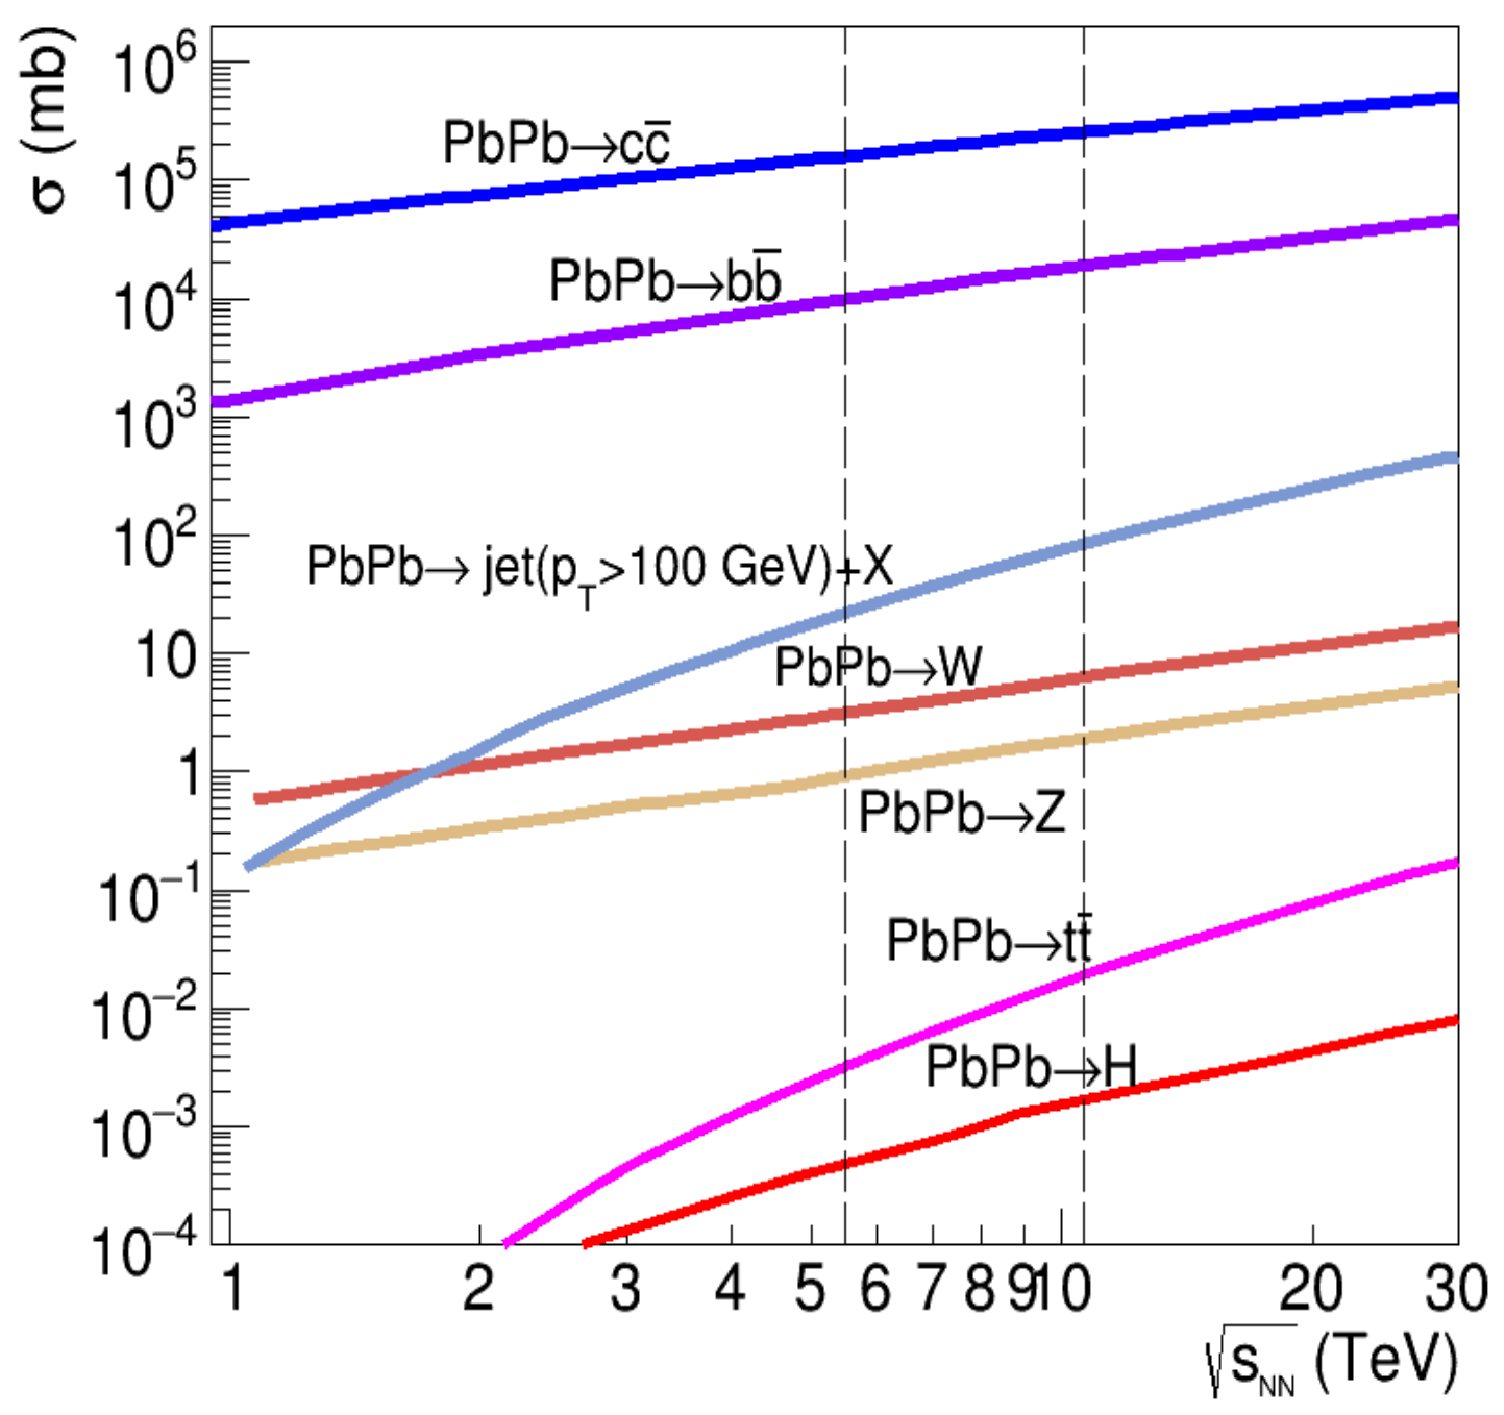
\includegraphics[width=0.5\textwidth]{helhc/figs/xsecVSsqrts.pdf}
\hfill
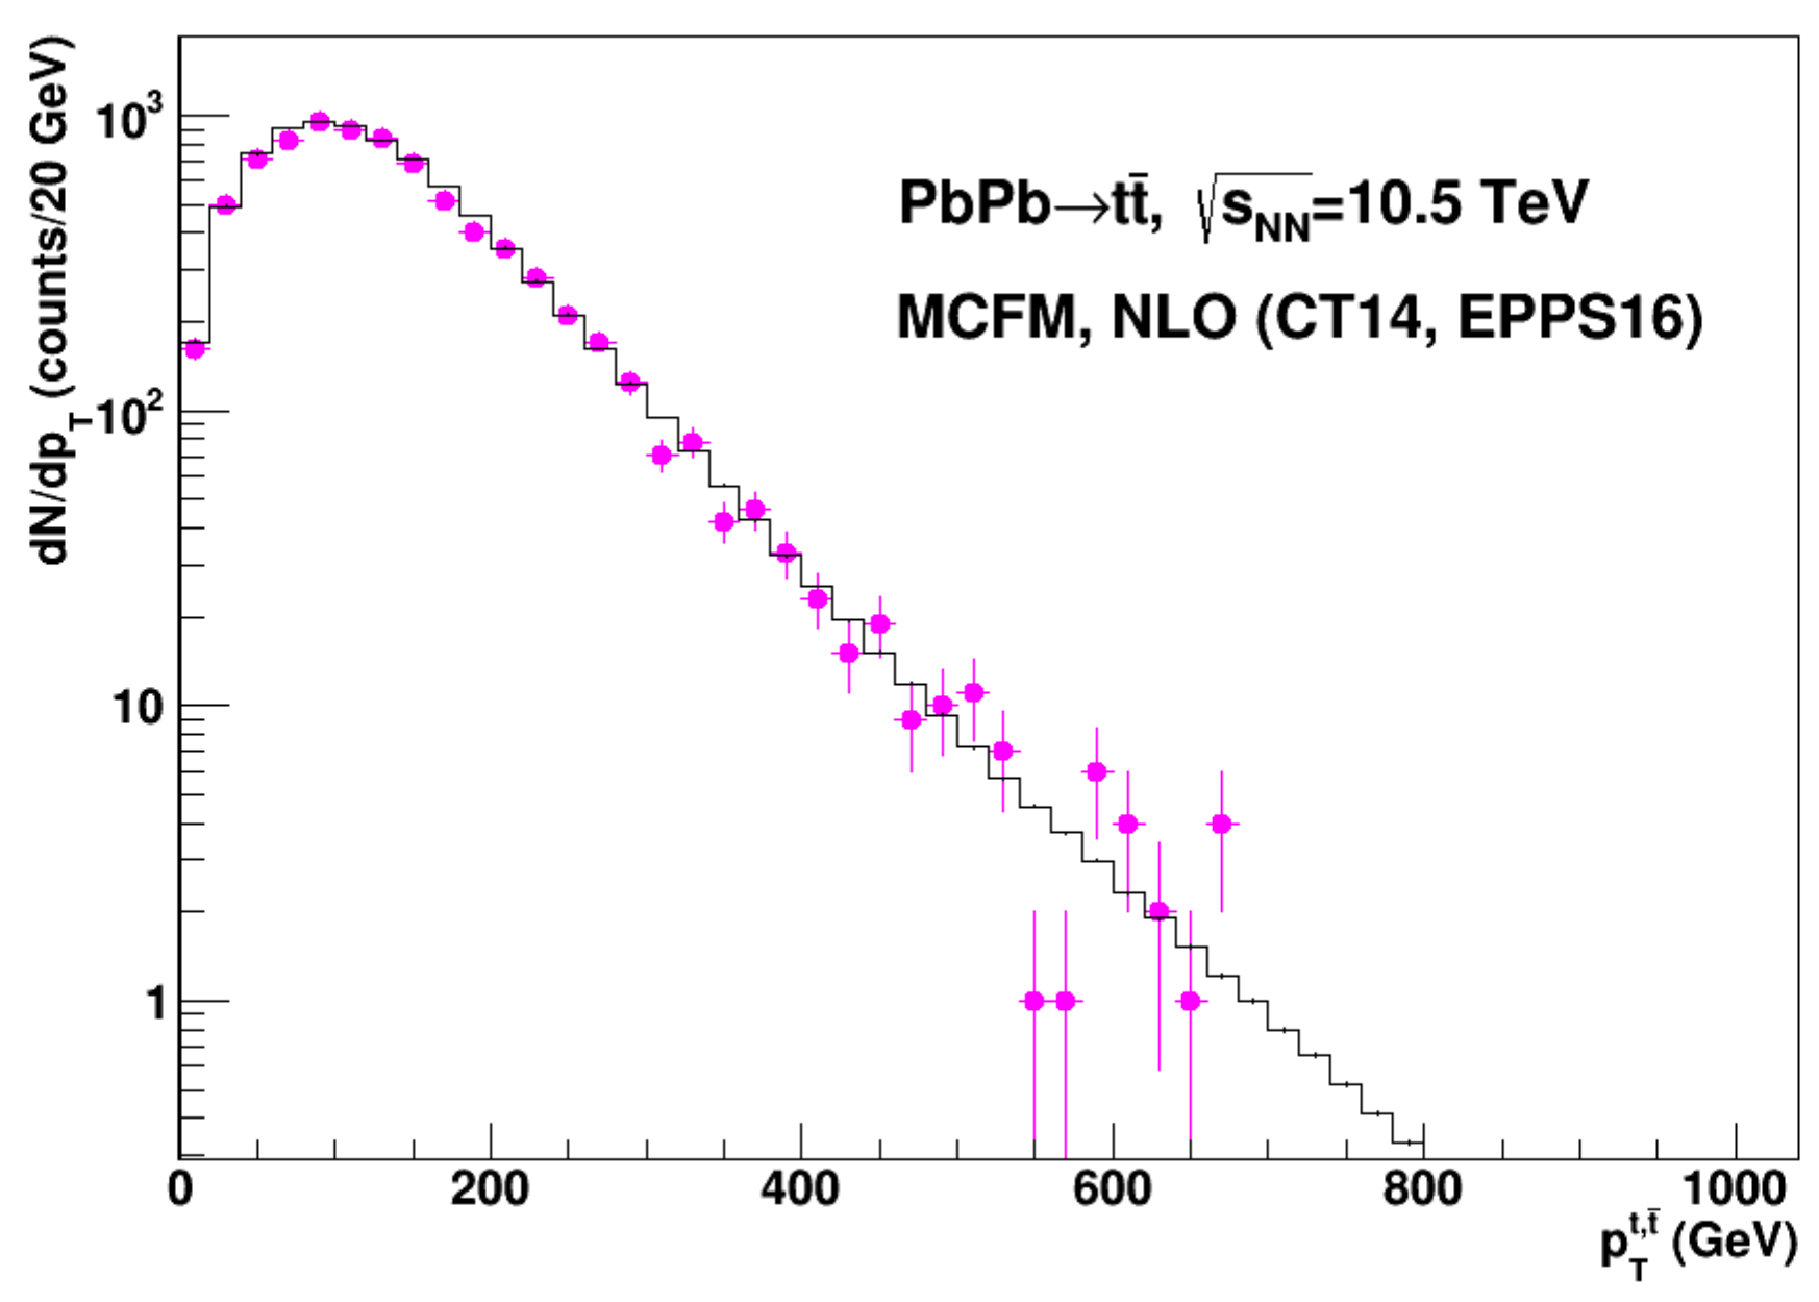
\includegraphics[width=0.48\columnwidth]{helhc/figs/toppT_HE_PbPb3nb.pdf}
\caption{Left:$\sqrt s$-dependence of the cross sections for hard processes of
  interest for a heavy-ion programme, calculated with MCFM~\cite{Campbell:2010ff}
at the highest available order. 
  Right: Expected top-quark $\pt$ distribution in \PbPb\ in the
  decay channels of interested for boosted top analysis at $\sqrtsnn=10.6$~TeV after acceptance and
  efficiency cuts with the statistical uncertainties
  for $L_{\rm int}=3$~nb$^{-1}$ {\bf to be redone for 3 months: 18/nb} (adapted from~\cite{dEnterria:2015mgr}).}
\label{fig:hardXsectHIC}
\end{center}
\end{figure}





The motivations for measurements of top quarks in heavy-ion collisions
are multifold, {\bf as discussed in Sections~\ref{sec:top4npdfs} and ArAr} . For example, in
p--Pb collisions the cross sections efficiently probe the nuclear
gluon PDFs in a wide range in momentum fraction
$x$ at high scale $Q\sim m_{\rm t}$~\cite{dEnterria:2015mgr} (see Section~\ref{sec:top4npdfs}). In Pb--Pb
collisions, the top-quark observables are sensitive to the energy-loss of heavy quarks~\cite{Baskakov:2015nxa}
and by selecting boosted (very high-$p_{\rm T}$) top quarks one could also probe the QGP medium at later times as the decays of boosted top quarks get Lorentz
time dilated (see next section). 
For example, the estimated measurable yields  for $t\bar t\to b\bar b\,\ell\ell\,\nu\nu$ (using the
 per-month luminosities discussed in Section~\ref{sec:HELHC_intro}) with
realistic analysis cuts 
and conservative 50\% efficiency for $b$-jet tagging are
about $10^4$ in Pb--Pb collisions and $3\times 10^4$ in Xe--Xe collisions (for the case of three-fold increase of NN integrated luminosity with respect to Pb--Pb).

As mentioned above, the $p_{\rm T}$ reach of top quarks in Pb--Pb collisions is of special importance for QGP
studies. Figure~\ref{fig:hardXsectHIC} (right) shows the estimated $p_{\rm T}$ spectrum
of the yields {\bf (per month)} in Pb--Pb collisions for top-quark pair production. The figure indicates that one
could measure top quarks approximately {\bf up to $p_{\rm T} \approx
1.8~{\rm TeV}/c$, even considering only one run in the baseline
luminosity scenario. At mid-rapidity, $p_{\rm T}$ as large
as this would correspond approximately to a factor of 10 time dilation
in the top decay (see next section). }

Another potential novel probe of the QGP medium at FCC energies is the
Higgs boson. The Higgs boson has a lifetime of $\tau\approx 50$~fm/$c$, which is much larger than the 
time extent of the QGP phase. It has been argued that the Higgs boson
interacts strongly with the quarks and gluons of the QGP and the interactions
induce its decay in the gluon--gluon or quark--antiquark channels, thus depleting the 
branching ratio to the most common ``observation'' channels $\gamma\gamma$ or $ZZ^\star$~\cite{dEnterria:2018bqi}.
%The amount of Higgs boson ``suppression'' in these channels is estimated to be of about 15\% for $p_{\rm T}<50~{\rm GeV}/c$ and to vanish above 100~GeV/$c$.
This ``suppression'' could potentially be used 
to accurately determine the final-state density of the produced QGP.
The cross section for Higgs boson production in Pb--Pb collisions is expected to
increase by a factor about 4 when going from
$\sqrtsNN=5.5~\tev$ to $\sqrtsNN=10.6~\tev$~\cite{dEnterria:2017jyt}.
A statistically-significant Higgs boson observation in the
$\gamma\gamma$ decay channel in Pb--Pb collisions at HE-LHC 
requires an integrated luminosity of $>70$~nb$^{-1}$ 
(estimated as in Ref.~\cite{dEnterria:2017jyt}), which corresponds to about 14 months with the present machine performance
projections. With Xe--Xe collisions the same statistical significance could be reached in 4 months.


\subsubsection{Boosted tops and the space-time picture of the QGP}
\label{sec:HE_boostedtops}

The HE-LHC would provide large rates of highly-boosted heavy particles, such as tops, $Z$ and $W$ bosons. It is expected that when these particles decay the density profile of the QGP has already evolved. It has been argued that the hadronically-decaying $W$ bosons in events with a $t\bar t$ pair can provide unique insights into the time structure of the QGP~\cite{Apolinario:2017sob}. This is because the time decays of the top and the $W$ bosons are followed by a time-delay in the interaction of the decay products of the $W$ boson with the surrounding medium due to a color coherence effect. The sum of the three times, that reaches values of several fm/$c$ for boosted tops, would be the time at which the interaction with the QGP begins, providing a unique way to directly measure the time structure of the QGP evolution.
In addition, due to colour coherence effects, energy loss  would be initially absent for the colour-singlet $q\overline q$ decay products of a highly-boosted $W$ boson: the two quarks would start to be quenched only when their distance becomes larger than the colour correlation length of the medium, which depends on the transport coefficient $\hat{q}$ (the average transverse momentum squared that particles exchange with the medium per unit mean-free path)~\cite{CasalderreySolana:2012ef}.
The effect on the reconstructed masses of the top and $W$ is studied, for $t\bar t$ events decaying semileptonically, with different energy loss scenarios as a proof of concept of the potential of these observables to access completely novel quantities in heavy-ion collisions. Times in the range $0.3$--$3$~fm/$c$ are obtained when adding the time delay from Lorentz boosts of the decaying top quark and $W$ boson and the time in which a singlet antenna remains in a colour coherent state~\cite{Apolinario:2017sob}. 


\begin{figure}[!t]
\begin{center}
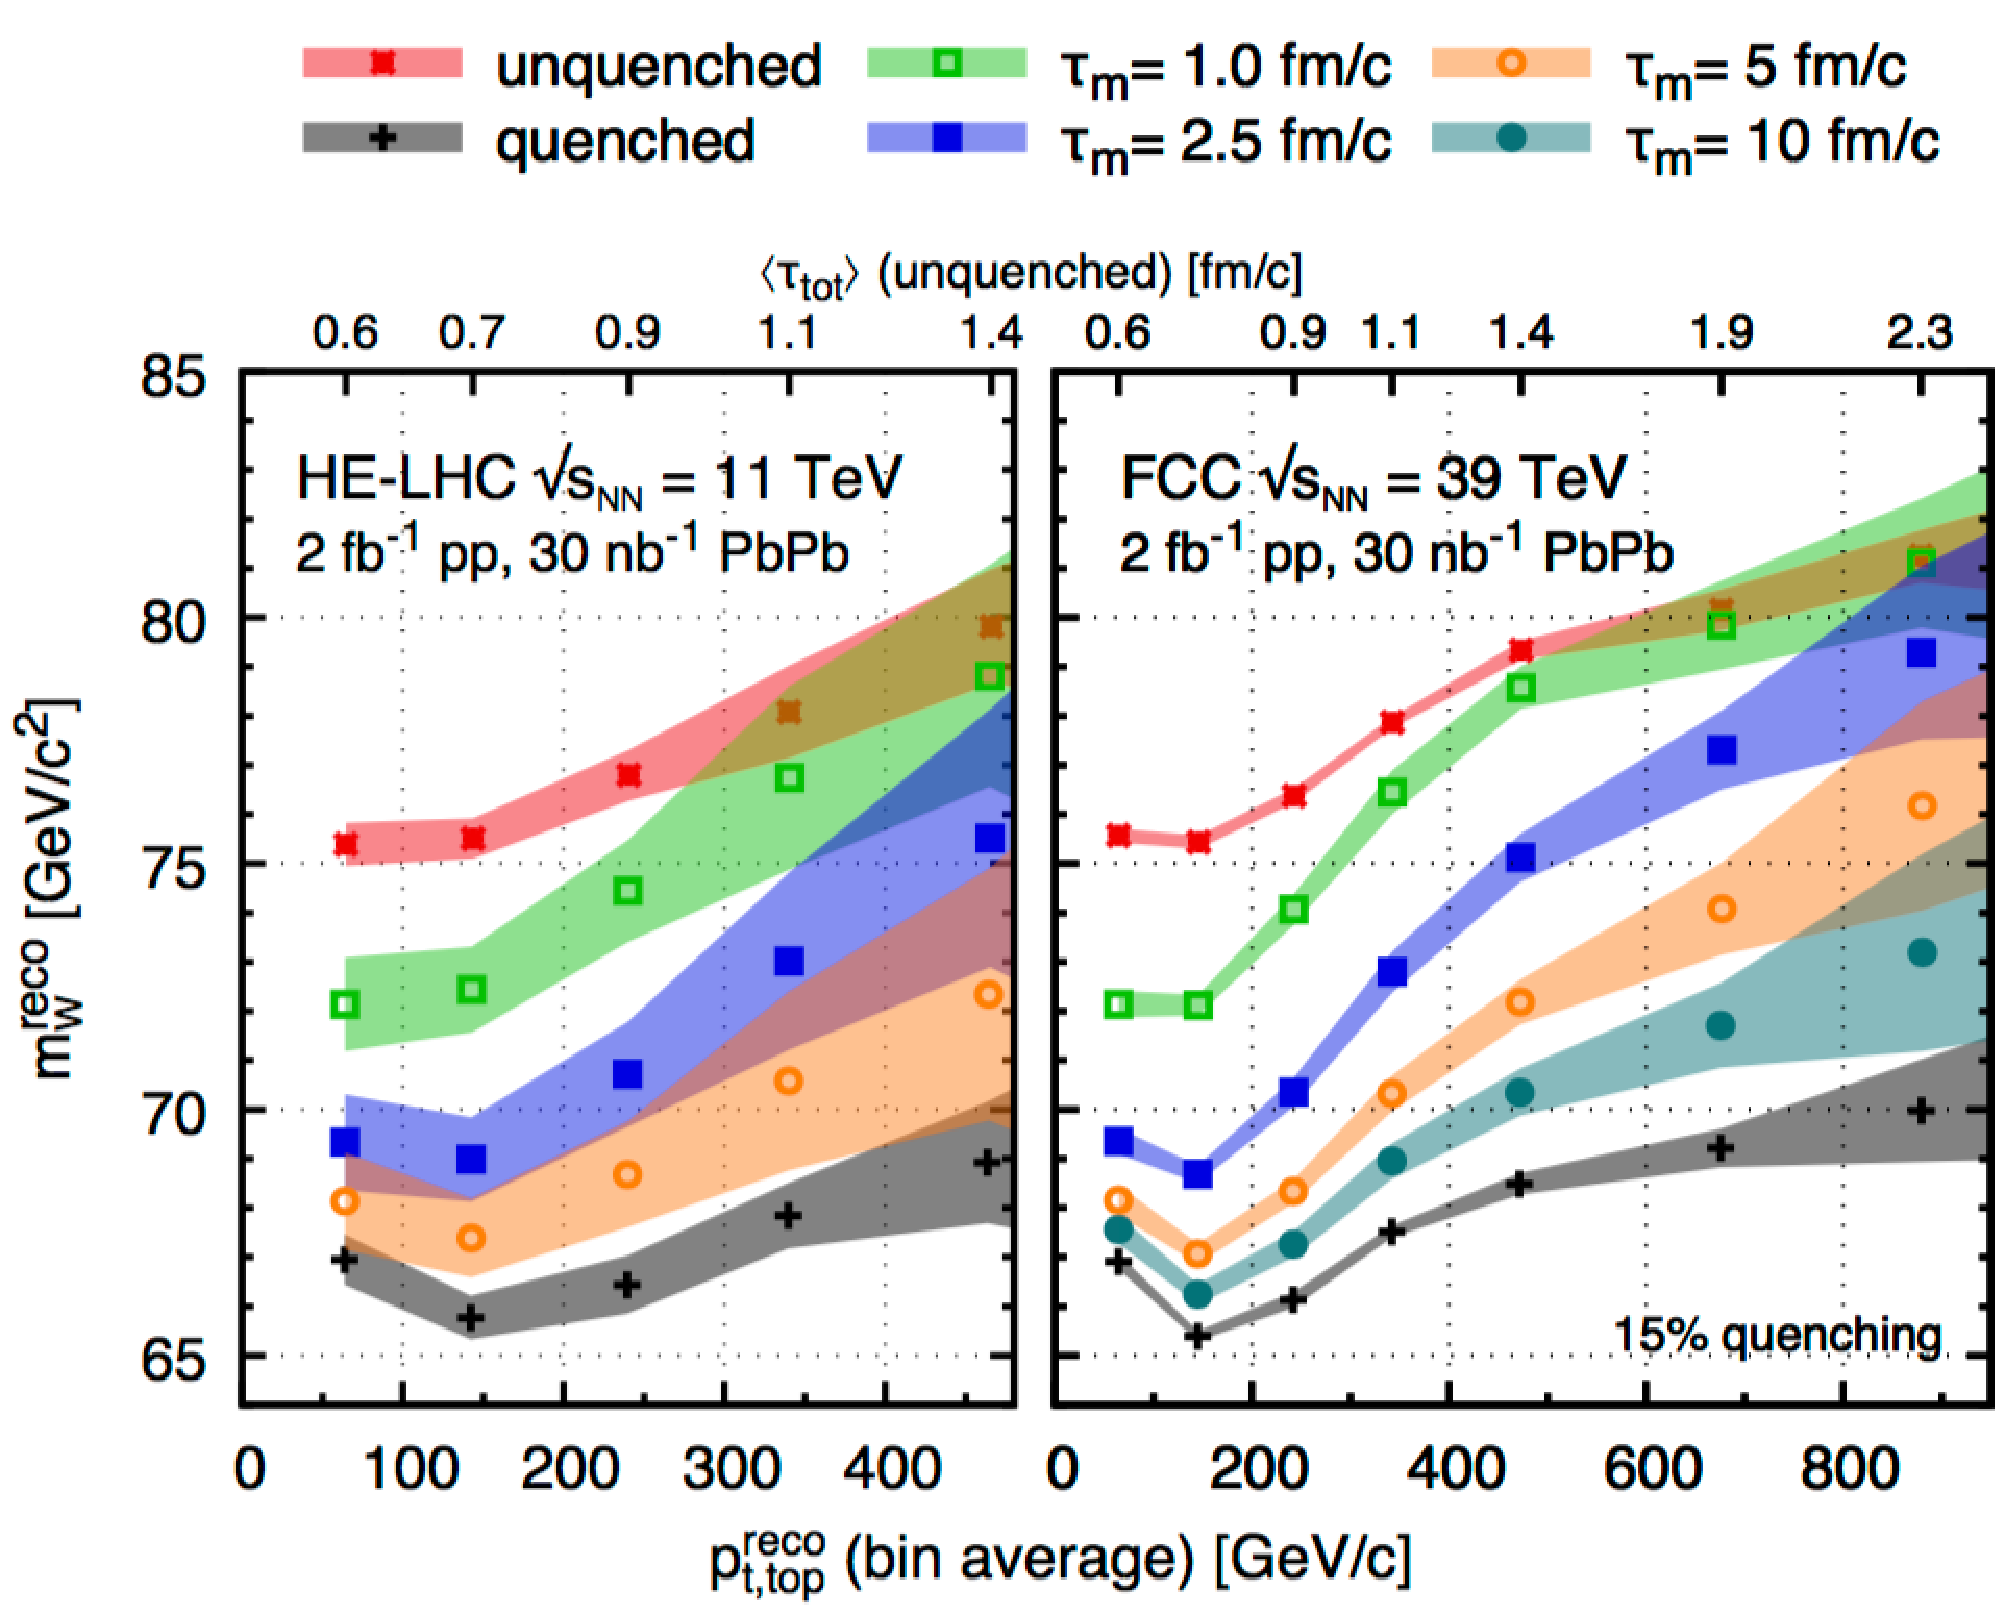
\includegraphics[width=0.46\textwidth]{helhc/figs/WMass_tops.pdf}
\hfill
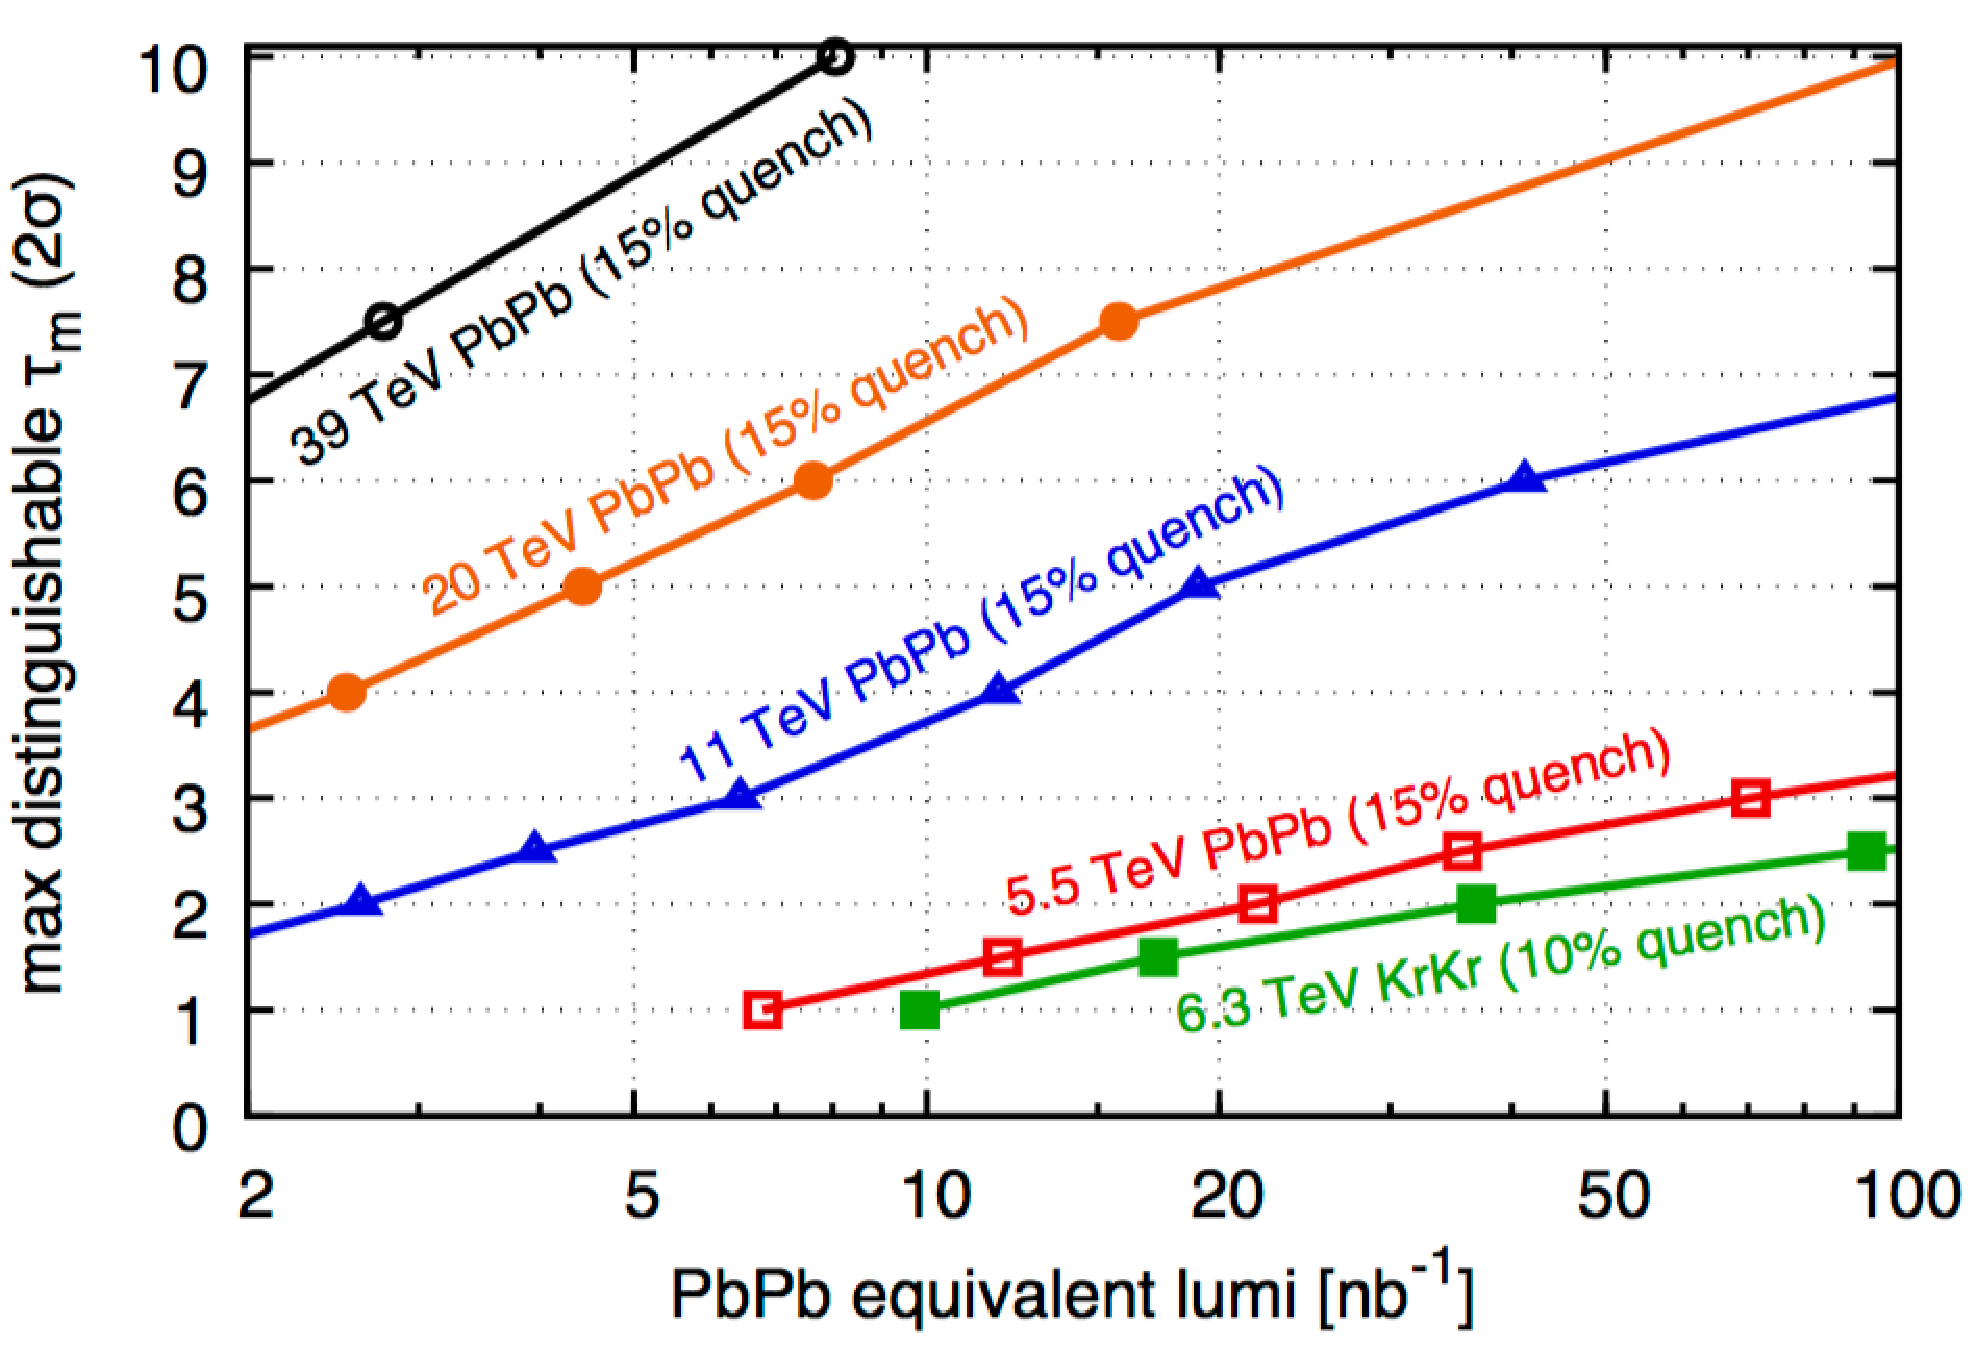
\includegraphics[width=0.5\textwidth]{helhc/figs/Taum_tops.pdf}
\caption{Left: Reconstructed $W$ boson mass at HE-LHC and FCC
  energies, as a function of the top $\pt$. The upper axis refers to
  the average total time delay of the corresponding top $\pt$
  bin. Right: maximum medium quenching
end-time, $\tau_m$, that can be distinguished from full quenching with
two standard deviations, as a function of luminosity for various
collider energies and species. Figures from Ref.~\cite{Apolinario:2017sob}. {\bf Curves for XeXe and KrKr at HE-LHC to be added.} }
\label{fig:tops}
\end{center}
\end{figure}


The reconstructed $W$-boson mass as a function of top transverse
momentum at $\sqrtsNN = 11$~TeV is shown in Fig.~\ref{fig:tops}
(left), together with the FCC case. For details on the simulation and reconstruction procedure
see~\cite{Apolinario:2017sob}. 
The shaded region corresponds to the statistical uncertainty obtained
with a bootstrap analysis considering central Pb--Pb collisions for
$L_{\rm int} = 30$~nb$^{-1}$ (corresponding to 5 Pb--Pb months or 1.5 Xe--Xe months with the present luminosity estimates)
and $L_{\rm int} = 2$~fb$^{-1}$ for the pp reference.
Energy loss was simulated considering that all particles, except the $W$ boson decay products, lose $15\%$ of their initial momentum. 
Average time delays $\tau_m = 1; 2.5; 5$ and $10~$fm$/c$ were considered as effective QGP time evolution profiles. 
Fig.~\ref{fig:tops} (right) shows the maximum medium quenching
end-time, $\tau_m$, that can be distinguished from full quenching with
two standard deviations, as a function of luminosity for various
collider energies and species. For Pb--Pb with $L_{\rm int}=30$~nb$^{-1}$ (5 months) 
at HE-LHC a maximum time of 5--6~fm/$c$ can be accessed, which is much
larger than the time up to 1.5~fm/$c$ that can be probed at the LHC with the nominal programme of 
10~nb$^{-1}$. {\bf Elaborate about Xe-Xe case.}


\subsubsection{Heavy flavour and quarkonia}
\label{sec:HE_hf}


Heavy quarks (charm and bottom) are among the hard probes that have
provided important insights on the formation and the characterics of
the QGP, see Section~\ref{sec:HI_HF} and Ref.~\cite{Andronic:2015wma}.
%On the one hand, quarkonium states are sensitive to the formation and to the
%temperature of a deconfined plasma via the mechanism of colour-charge
%screening, which is thought to be to some extent balanced by the
%recombination of heavy quarks and antiquarks from the plasma.
%On the other hand, the production of hadrons with open heavy flavour
%is sensitive to the QGP-induced modification of the momentum value and
%direction of heavy quarks, thus providing
%insight on the interaction mechanisms of heavy quarks
%with the constituents of the QGP and on its
%transport properties.
In this section,
a few selected aspects that could
represent novel or particularly remarkable observations at HE-LHC
energy are discussed,
namely: i) large production of thermal charm from
  interactions of light quarks and gluons within the QGP;
ii) observation of an enhancement of charmonium production with
  respect to the binary scaling of the yields in pp collisions, as
  consequence of (re)generation;
iii) observation of a colour screening and (re)generation for the most tightly-bound
  quarkonium state, the $\Upsilon$(1S).

Interactions between gluons or light quarks of the QGP can lead to the
production of $c\overline c$ pairs if the energy in the centre of mass 
of the interaction is of the order of twice the charm quark mass
$\sqrt{\hat s}\sim 2\,m_c\sim 3$~GeV. 
In Section~\ref{sec:HE_qgpglobal} we have estimated 
that an initial temperature $T_0$ of 600--800~MeV could be
reached at the HE-LHC. 
With these QGP temperatures a sizeable fraction of the gluons and
light quarks have energies larger than the charm quark mass 
and $c\overline c$ pairs can be produced in their interactions. 
Figure~\ref{fig:thermalcharm} shows the prediction~\cite{Liu:2016zle} for the time-dependence of the $c\overline c$
rapidity density at mid-rapidity in central Pb--Pb collisons at HE-LHC. The value at the initial time
$\tau_0$ corresponds to the initial hard-scattering cross section.
Both calculations show a rapid increase
after $\tau_0$ with a final value that is larger by up to 20\% than
the initial production. 
This enhancement could be for the first time observed at the HE-LHC
and provide a handle on the initial
temperature of the QGP. 
The abundance of charm quarks also has an effect on the QGP equation
of the state: 
the inclusion of the charm quark in the lattice QCD calculations results in a sizeable 
increase of $P/T^4 \propto n_{\rm d.o.f.}$ for $T>400$~MeV, as
discussed in the context of the FCC~\cite{Dainese:2016gch}.  

\begin{figure}[!t]
\begin{center}
%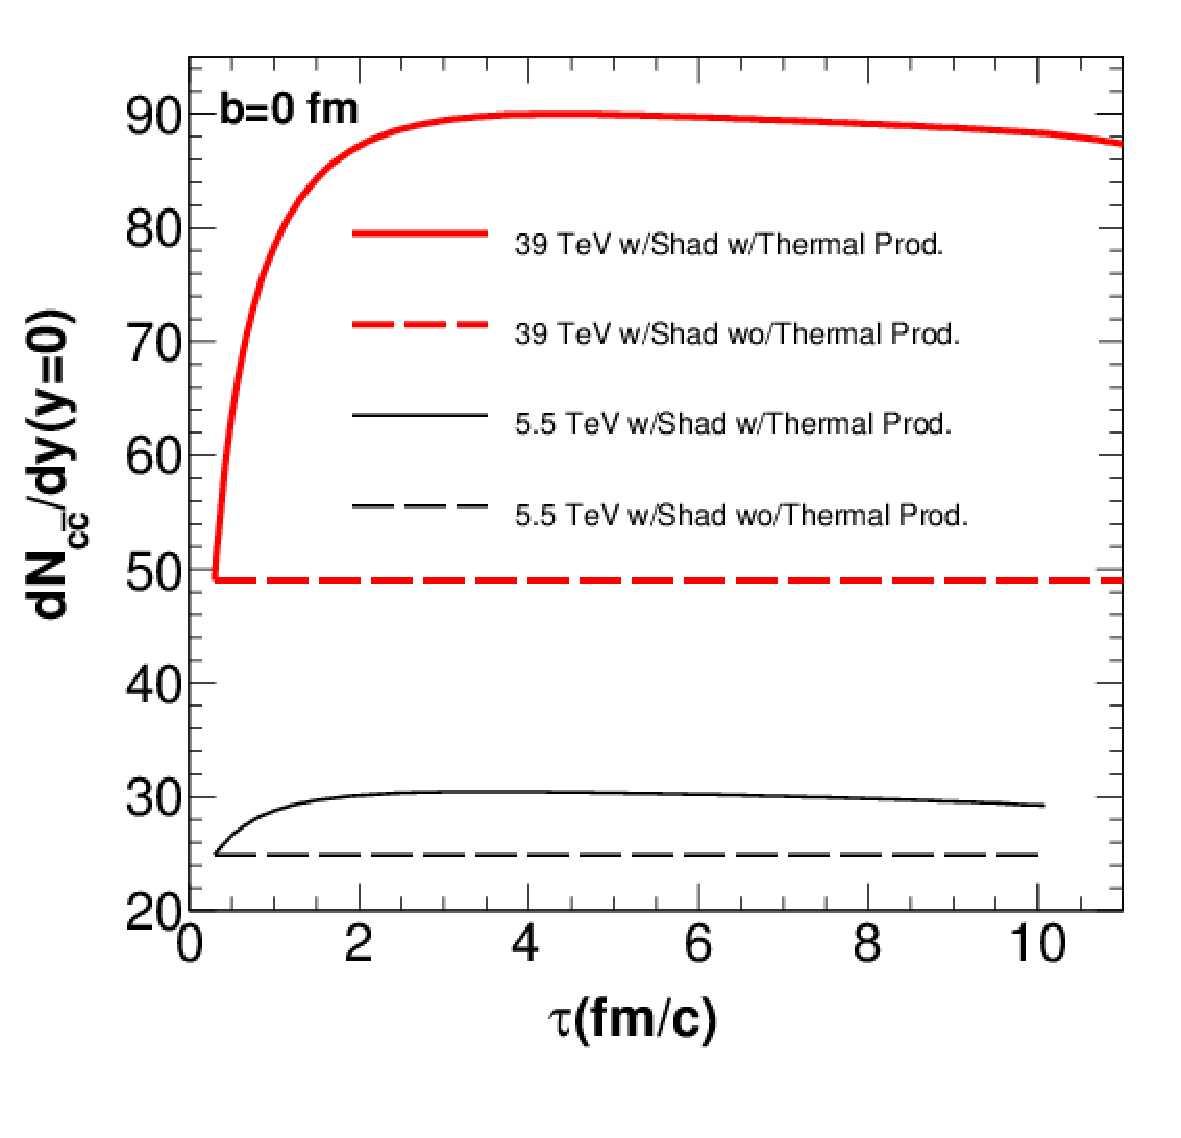
\includegraphics[width=0.42\textwidth]{helhc/figs/charmZhou.pdf}
%\hfill
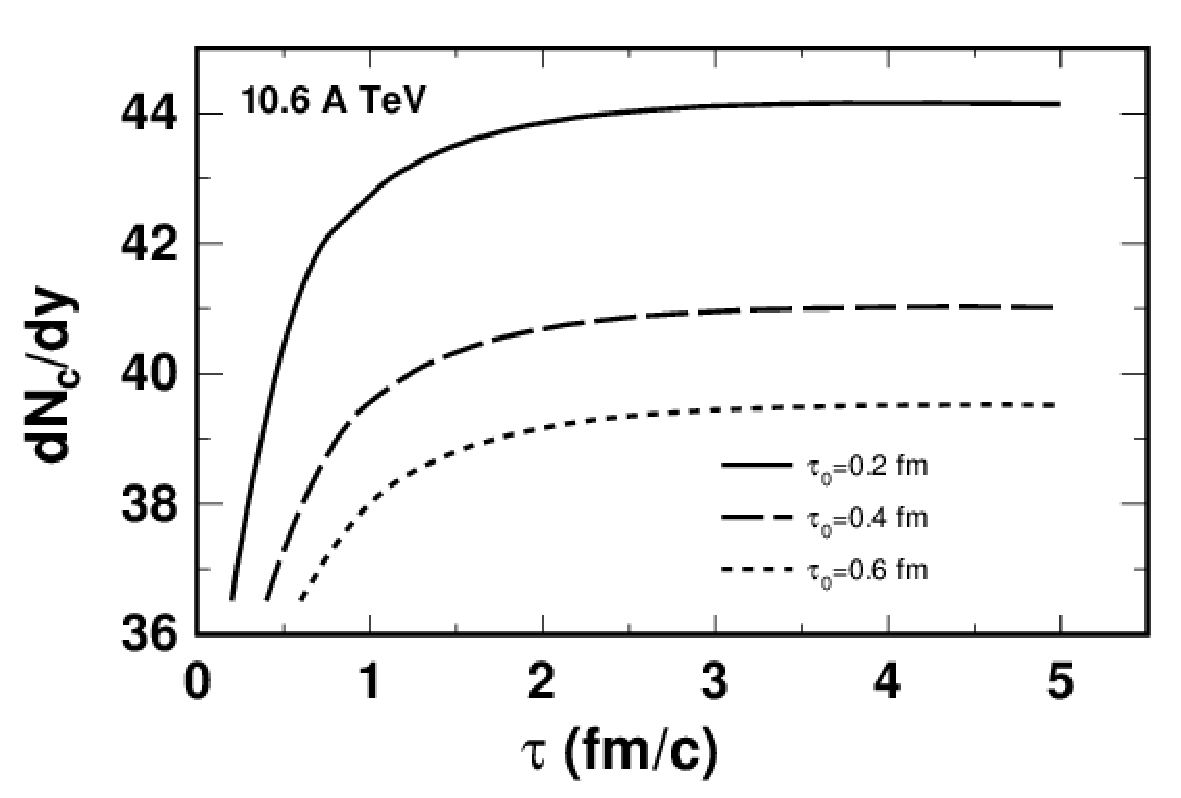
\includegraphics[width=0.54\textwidth]{helhc/figs/charmKo_PbPbHE.pdf}
\caption{Time-evolution of the $c\overline c$ yield
  (per unit of rapidity at midrapidity) for central Pb--Pb collisions
  at $\sqrtsNN=10.6$~TeV, obtained as described in Ref.~\cite{Liu:2016zle}.}
\label{fig:thermalcharm}
\end{center}
\end{figure}




The measurements of the nuclear modification factor of J$/\psi$ at the LHC~\cite{Adam:2015isa,Adam:2015rba,Chatrchyan:2012np} 
are described by models that include dissociation caused by
colour-charge screening and a contribution of recombination
(usually denoted (re)generation) from deconfined $c$ and $\overline c$
quarks in the QGP~\cite{Liu:2009nb,Zhao:2011cv,Andronic:2011yq}. 
The (re)generation contribution is expected to be proportional to
the rapidity density of $c\overline c$ pairs in the QGP. 
Therefore, it is predicted to be much larger
at HE-LHC than LHC energies, as a consequence of the larger hard-scattering
production cross section of $c\overline c$ pairs and the possible 
sizeable thermal production.
This could lead to the observation of an enhancement of J$/\psi$
production with respect to binary scaling of the yield in pp
collisions, i.e.\,$R_{\rm AA}>1$, which would be a striking evidence of 
$c\overline c$ recombination from a deconfined QGP.

%Figure~\ref{fig:oniaRAA} (left) shows the predicted J$/\psi$ $\RAA$ at FCC
%energy, as obtained with the Statistical Hadronization
%Model~\cite{jpsiFCCshm}. 
%The model predicts $\RAA(\pt>0)>1$ in central collisions and an
%increase of about 40\% with respect to top LHC energy.

%\begin{figure}[!t]
%\begin{center}
%\includegraphics[width=0.42\textwidth]{figs/JpsivsnpartSHM.pdf}
%\hfill
%\includegraphics[width=0.42\textwidth]{figs/Raa_npart_Y1S_40_y0.pdf}
%\caption{Nuclear modification factor $\RAA$ of J$/\psi$ (left) 
%and $\Upsilon(1S)$ mesons (right)
%at LHC and FCC energies as a function of the collision centrality
%(number of participant nucleons)~\cite{Andronic:2011yq,jpsiFCCshm}.}
%\label{fig:oniaRAA}
%\end{center}
%\end{figure}


The measurement of $\Upsilon$ production would be particularly interesting
at the high
energies and temperatures reached at the HE-LHC.
The LHC data are consistent with a scenario in which the excited
states 2S and 3S are partially or totally suppressed by colour
screening, while the 1S, which is the most tightly bound state, has no
or little direct melting. Its suppression by about 50\% can be
attributed to the lack of feed-down from the (melted) higher states
(see e.g.\,Ref.~\cite{Andronic:2015wma} for a recent review).
At HE-LHC energies, on the one hand, the temperature could be large
enough to determine a full melting even of the tightly-bound 1S state,
on the other hand the large abundance of $b\overline b$ pairs in the
QGP could induce substantial $\Upsilon$ (re)generation.
%The possibly large effect of (re)generation of bottomonia from $b$
%and $\overline b$ quarks 
%is illustrated by the prediction of the Statistical
%Hadronization Model~\cite{Andronic:2011yq,upsilonFCCshm} for the $\RAA$ of $\Upsilon$(1S) as a function of centrality, shown in the right panel of  
%Fig.~\ref{fig:oniaRAA}. 
%The predictions are calculated for values of
%$d\sigma_{b\overline b}/dy$ in nucleon--nucleon collisions ranging 
%from 73 to 163~$\mu$b, as obtained at NLO~\cite{Mangano:1991jk},
%which result in 15--40 $b\overline b$ pairs
%in central Pb--Pb collisions.
%The resulting $\Upsilon$(1S) $\RAA$ in central Pb--Pb collisions is predicted
%to range between 0.3 and 1.2.
The role of the two effects ---degree of survival of initial bottomonia and contribution of
(re)generation--- could be separated by means of precise measurements of
the $b\overline b$ cross section
and of the $B$ meson and $\Upsilon$ $\RAA$ and elliptic flow $v_2$ 
(the regenerated $\Upsilon$ states could exhibit a $v_2$ such that $0<v_2^{\Upsilon}<v_2^B$).

  
\subsection{Nuclear PDF measurements and search for saturation}
\label{sec:HE_smallx}

\newcommand{\pizero}{\ensuremath{\pi^{0}}}
\newcommand{\ptjet}{\ensuremath{p_\mathrm{T,jet}}}


%\subsubsection{Small-$x$ PDFs, factorisation, saturation}
%\label{sec:HI_smallxintro}

Parton saturation~\cite{Gribov:1984tu,Mueller:1985wy} is based on the idea that standard linear parton branching  leads, at small values of momentum fraction $x$, to parton densities so high that non-linear dynamics (like gluon recombination) becomes important and parton densities are tamed to grow from power-like to logarithmically. Non-linear effects are expected to become important when the density of gluons per unit transverse area exceeds a certain limit, the \textit{saturation density}. 

In the framework of QCD collinear factorization, Parton Distribution Functions of nucleons inside nuclei (nuclear PDFs) can be obtained in standard global fit analysis with usual linear evolution equations. 
The differences with respect to free nuclon PDFs are parametrized in a nuclear modification factor
$R_i^{\rm A}(x,Q^2)$ with $i=g,\,q_{\rm valence},\,q_{\rm sea}$ (see e.g.\,Ref.~\cite{Arneodo:1992wf}).
Collinear factorization 
is expected to break down when the gluon phase-space becomes saturated.
%In these conditions, 
%the small-$x$ partons in the nuclear wave function would
%act coherently, not independently as assumed with factorization.
%The Color Glass Condensate (CGC) is the non-perturbative, but weak coupling description of such a system, which relies on resummation of powers of parton density (see e.g.\,Ref.~\cite{Gelis:2010nm}).
The onset of saturation is usually discussed in terms of the 
saturation momentum $Q_{\rm S}^2$, defined as the 
scale at which the transverse area of the nucleus is completely saturated and gluons start to overlap.
It can be shown that $Q^2_{\rm S} \sim {A}^{1/3} \big(\sqrtsNN\big)^\lambda e^{\lambda y}$,  with $\lambda \approx 0.3$~\cite{Dainese:2016gch}.
%Saturation affects the processes in the region $Q^2\,\lsim\, Q^2_{\rm S}$.
Therefore, the regime of high gluon density is best accessed at a high-$\sqrtsNN$ hadron 
collider  with measurements at low $\pt$ and forward rapidity, which probe small $x$ and small $Q^2$.
%At present, no conclusive evidence has been provided for the existence of parton saturation, although a number of observations are consistent with its expectations~\cite{Dainese:2016gch}.
In order to firmly establish the existence of this new high-energy regime of QCD and clarify the validity of the different approaches to factorisation and evolution, new kinematic regions must be explored using higher collision energies in order to have a large lever arm in $Q^2$ in a region that, while perturbative, lies inside the saturation domain. The HE-LHC extends the small-$x$ coverage by a factor of two with respect to the LHC, as shown in Fig.~\ref{fig:kinplane}. 


\begin{figure}[h]
\centering
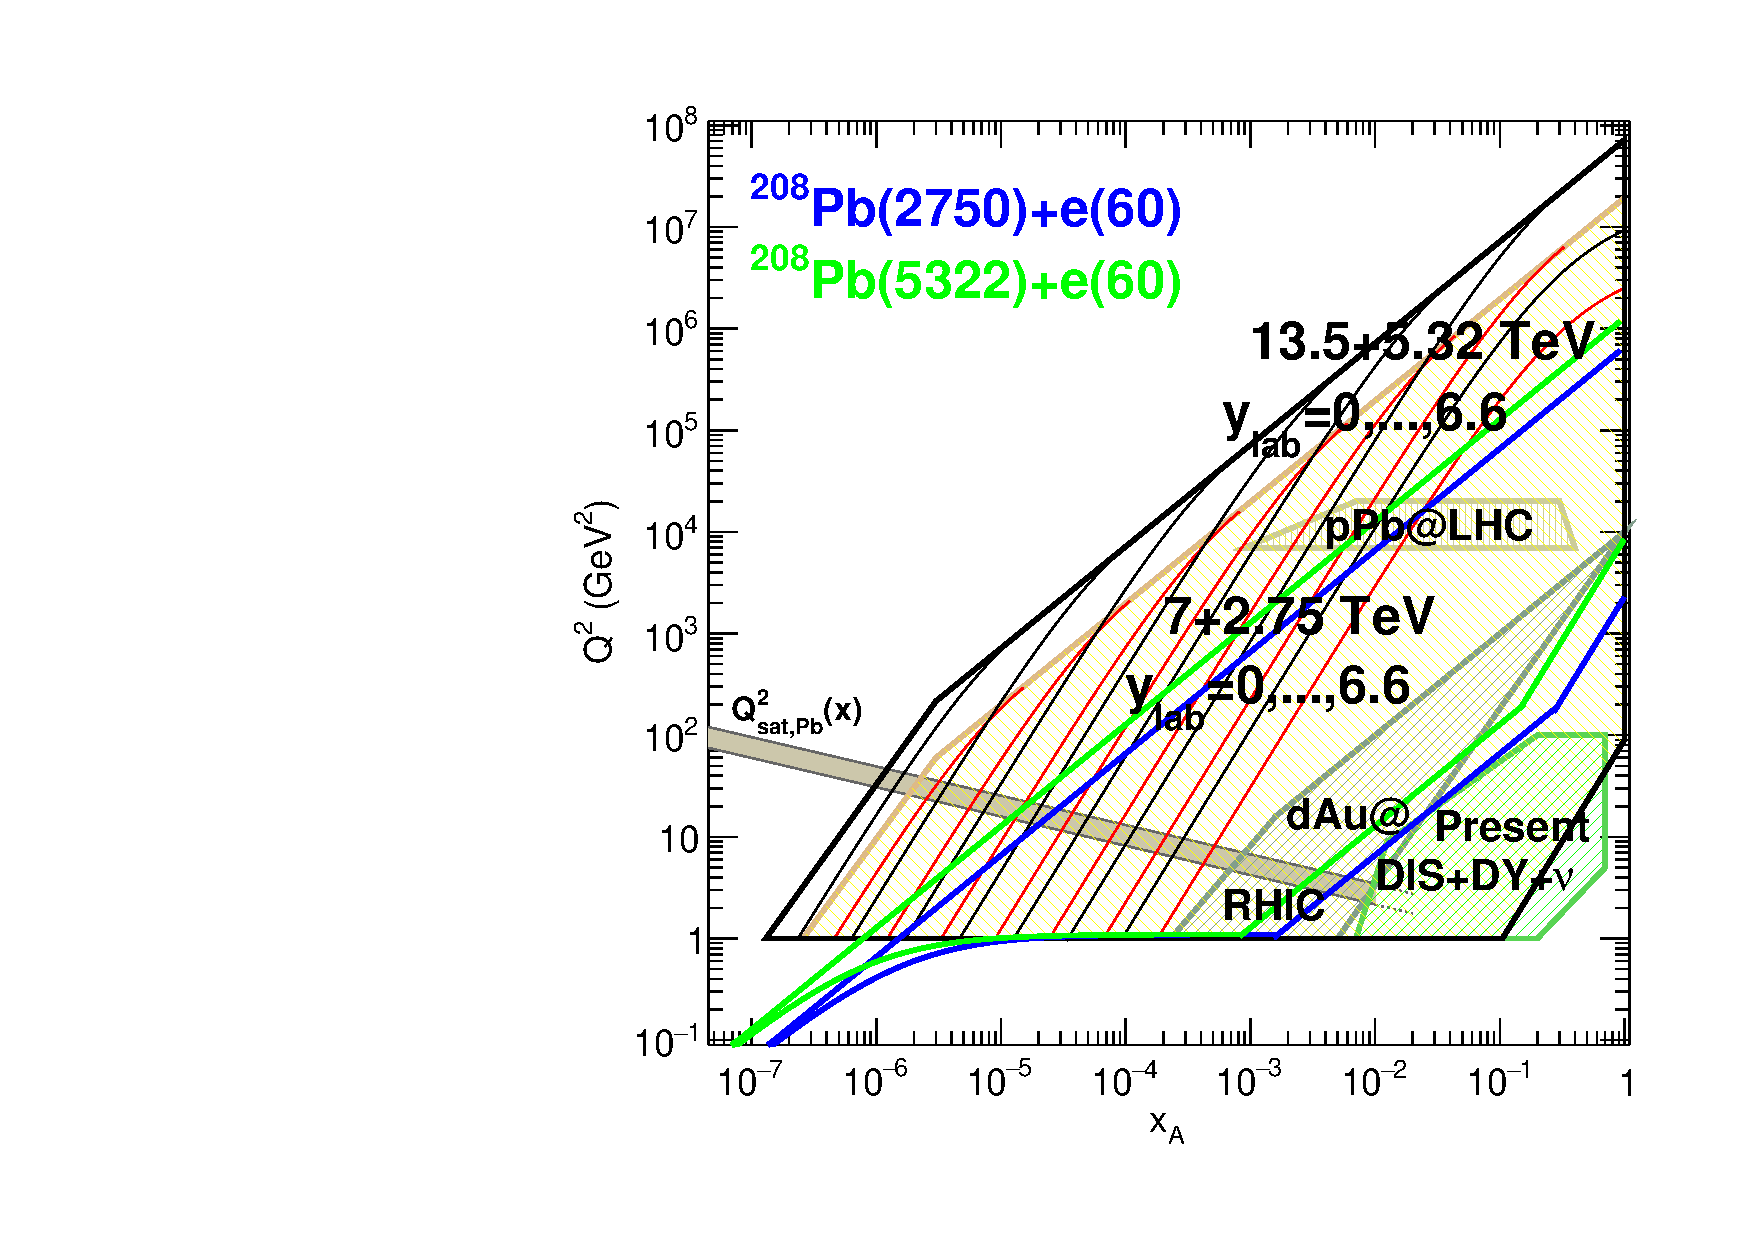
\includegraphics[width=0.55\textwidth]{helhc/figs/FHC8.pdf}
%\hskip 2cm\includegraphics[width=0.35\textwidth]{figs/Q2x_UPC_2.pdf}
\caption{Regions of the $x$--$Q^2$ plane covered %with presently available 
with nuclear DIS and Drell-Yan data and with p--A and e--A collisions at RHIC, LHC and HE-LHC.
For p--A  at the LHC and the HE-LHC, thin lines correspond to different rapidities in the
laboratory frame $y_{\rm lab} = 0$,1, 2, 3, 4, 5, 6 from right to left, with the left edge defined by $y_{\rm lab} = 6.6$. Values of $Q^2_{\rm S}(x)$ for Pb are shown for illustration.}
\label{fig:kinplane}
\end{figure}


There is a strong complementarity between the physics programmes at hadron colliders
and at the proposed electron--hadron colliders (Electron-Ion Collider in the USA~\cite{Accardi:2012qut}, Large Hadron Electron Collider LHeC~\cite{AbelleiraFernandez:2012cc}).
With kinematic reach at the TeV scale in the c.m.s.\,(Fig.~\ref{fig:kinplane}, left), 
the electron--nucleus option at HE-LHC would be well-positioned to reach conclusive evidence for the existence of a new non-linear regime of QCD. It would be clearly complementary with the p--Pb case, providing a precise knowledge on the partonic structure of nucleons and nuclei and on the small-$x$ dynamics. 


% \subsubsection{Searching for saturation with forward-rapidity photons and di-jets in p--A collisions}

% A full discussion of the observable sensitive to saturation at FCC-hh can found in the CERN Yellow Report~\cite{Dainese:2016gch}. Here we concentrate on two observables, both of which require measurements at forward rapidity $y\approx 4$ or larger: 
% single-inclusive spectra of photons and hadrons and azimuthal correlations of di-jets.

%  Single-inclusive measurements of charged hadrons, and photons and jets are the simplest observables that probe the gluon density. The two latter  are somewhat safer from a theoretical point of view, as they are free from hadronisation effects to a large extent.
% Photons are sensitive to the small-$x$ gluons via the dominant quark--gluon Compton scattering, as well
% as hadrons through underlying gluon--gluon scatterings that fragment into hadrons at moderate $\pt$ values.
% As shown in Fig.~\ref{fig:kinplane} (left),  measurements at mid-rapidity and $\pt < 10 \GeVc$ at the FCC potentially cover the saturation region with $Q\approx \pt$ and $x$ in the range $10^{-5}$--$10^{-4}$, which is at much lower $x$ and therefore larger gluon density than measurements at the LHC. Forward measurements, e.g.\,at $y \approx 4$, would be even more interesting, as they cover $x \approx 10^{-6}$.
% Figure~\ref{fig:marquet} (left) shows the ratios of $\pt$-differential cross sections of direct photons at rapidity 4 and 6 with respect to rapidity 2, calculated in the CGC framework~\cite{Rezaeian:2012wa,Rezaeian:2012ye}: saturation is expected to lead to a strong suppression for $\pt<10~\gev/c$ (the high-$\pt$ suppression at $\eta=6$ is an artifact of the calculation).

% Forward di-jets offer more potential to experimentally constrain the probed $x$ region, in particular at low \pt. CGC models predict a characteristic suppression of the recoil jet, because (mini-)jets can be produced by scattering a parton off the color field in the nucleus where the recoil momentum is carried by multiple gluons, unlike in a standard (semi-)hard 2-to-2 scattering where all the recoil momentum is carried by a single jet~\cite{Albacete:2010pg,Rezaeian:2012wa}.
% First measurements of di-hadron correlations at forward rapidity at RHIC show hints of the predicted suppression of recoil yield. However, the measurements are close to the kinematic limit and other mechanisms have been proposed to explain the suppression.  The FCC has a large potential for recoil measurements of hadrons, photons and jets, probing a broad range in $x$ and $Q^2$, while staying far away from the kinematic limit. 
% For di-jets at forward rapidity~\cite{vanHameren:2014lna,Kotko:2015ura}, 
% Fig.~\ref{fig:marquet} shows the expected broadening of the $\Delta\varphi$ distribution in p--Pb with respect to pp collisions (middle), as well as the expected nuclear modification factor for di-jets as a function of the transverse momentum of the leading jet \ptjet{}, in the recoil region (right).
%  A clear suppression is visible in the recoil region persisting to much larger $\ptjet > 100$~\GeVc{} than at the LHC, where the suppression is small at $\ptjet \approx 50$~\GeVc. These calculations clearly show  saturation effects up to high \pt, much larger than $Q_{\rm S}$, as long as the dijet transverse momentum imbalance does not exceed a few times $Q_{\rm S}$.

% \begin{figure}
% \centering
% \includegraphics[width=0.3\textwidth]{figs/plot-fcc-ratiof}\hfill
% \includegraphics[width=0.3\textwidth]{figs/pp_pPb_ITMD_dphi_35_45_63TeV}\hfill
% \includegraphics[width=0.3\textwidth]{figs/RpA_ITMD_pTmax_35-45_63TeV_Recoil}\hfill
% \caption{Left: ratio of direct photons at forward rapidities $\eta=2$, 4, 6 obtained in the CGC formalism in p--Pb collisions~\cite{Rezaeian:2012wa,Rezaeian:2012ye}.
% Middle: Forward di-jet $\Delta\varphi$ correlation in p--Pb compared to pp collisions at FCC~\cite{vanHameren:2014lna}. Left: nuclear modification factor of back-to-back di-jets at LHC and FCC energies.}
% \label{fig:marquet}
% \end{figure}



%\subsubsection{Constraining nuclear parton densities at large $Q^2$}
%\label{sec:HI_npdf}


Aside from the search for saturation at small-$x$ and $Q^2$, 
p--Pb and Pb--Pb collisions at HE-LHC would have strong potential for 
constraining nPDFs at large $Q^2$:
$W$ and $Z$ bosons, di-jets, top quarks. Here we will focus on the latter case, because it is a unique 
opportunity offered by the HE-LHC energy increase with respect to the LHC, and it offers 
the possibility to access in experimentally and theoretically well-controlled fashion the 
nuclear PDF at the unprecented large scale $Q=m_{\rm top}$~\cite{dEnterria:2015mgr,dEnterria:2017jyt}. 
{\bf To estimate the impact that the HE-LHC would have on nuclear gluon densities, the computed top-pair cross sections in
pp, p--Pb and Pb--Pb with analysis cuts (see~\cite{Dainese:2016gch}) have been binned in the rapidity $y_\ell$ of the $t\to W\to \ell$ decay leptons. 
Figure~\ref{fig:tnPDF} (left) shows Pb--Pb pseudodata for the expected nuclear modification
factors of the decay leptons. 
The effects that these, and the p--Pb, pseudodata would have in the EPS09~\cite{Eskola:2009uj} 
global fit of  nuclear PDFs are quantified via the
Hessian reweighting technique~\cite{Paukkunen:2014zia} and shown in the middle and right panels of the figure. The nPDF uncertainties are reduced by more than
50\% over a large range of $x$.}


\begin{figure}[ht]
\centering
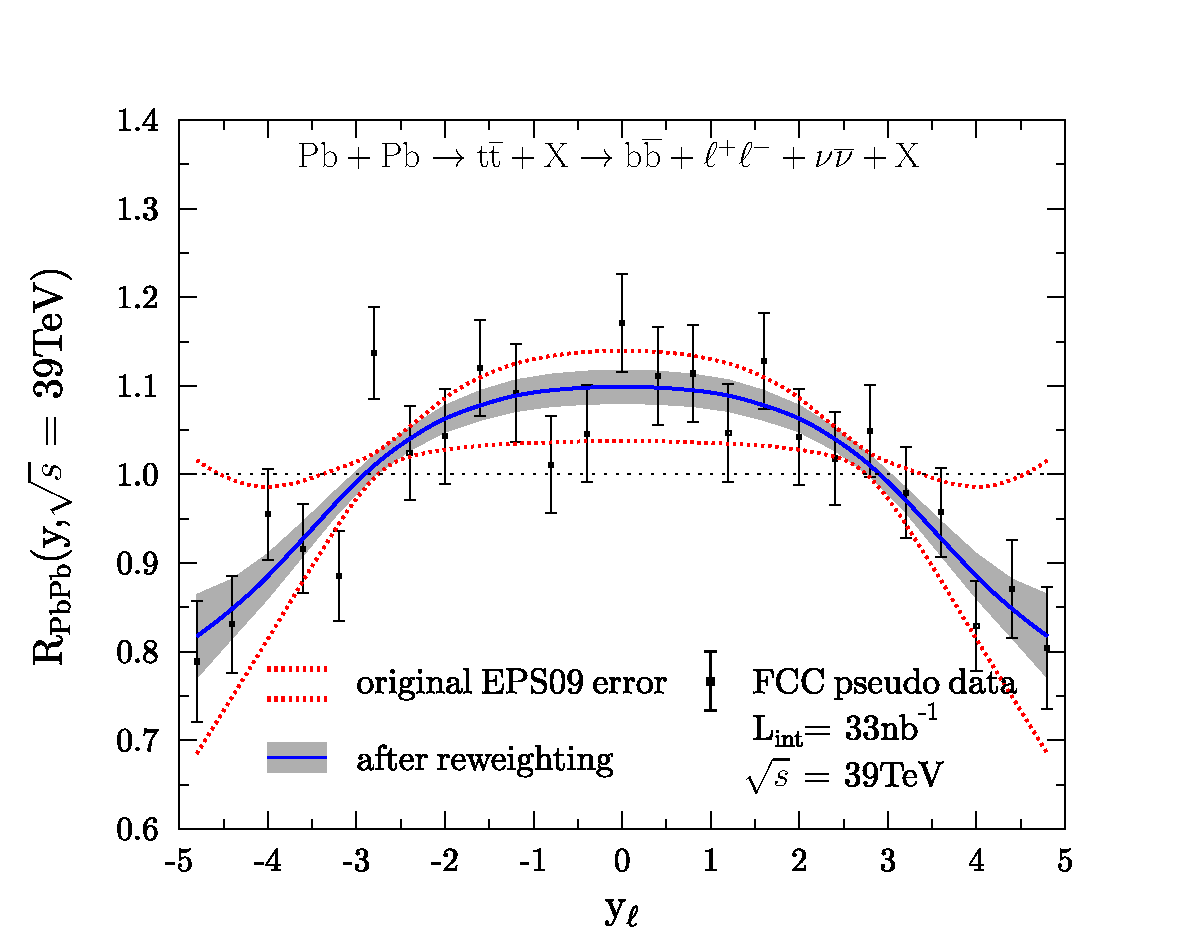
\includegraphics[width=0.325\textwidth]{helhc/figs/data3.pdf}
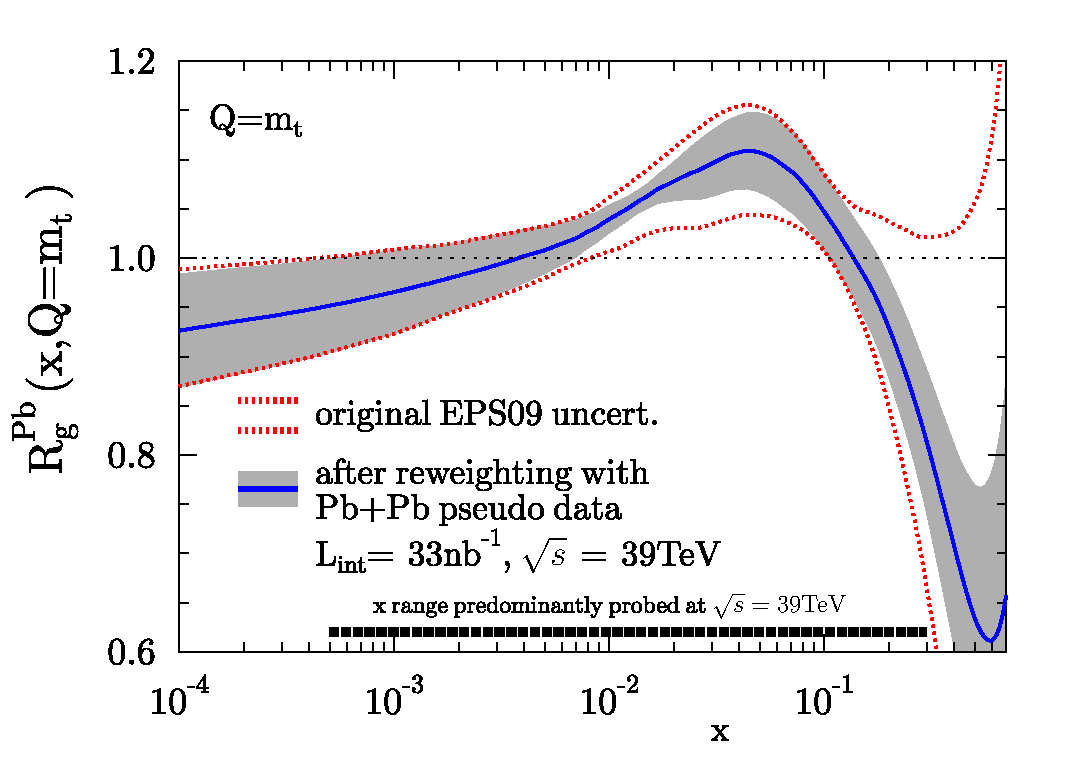
\includegraphics[width=0.33\textwidth]{helhc/figs/gluons3.pdf}
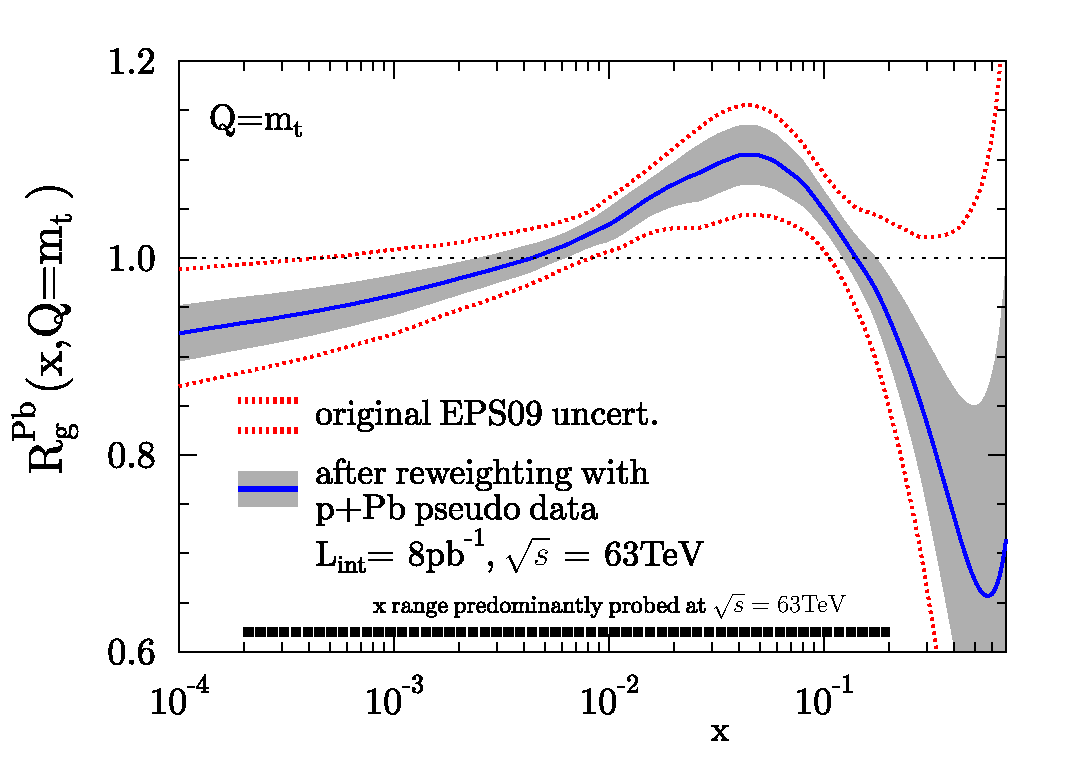
\includegraphics[width=0.33\textwidth]{helhc/figs/gluons4.pdf}
\caption{{\bf FIGS TO BE REDONE FOR HE-LHC ENERGY.} Left: HE-LHC pseudodata for the nuclear modification factor for top production in Pb--Pb collisions. Middle and right: Original EPS09 gluon nuclear modification  at $Q=m_{\rm top}$ and 
  estimated improvement obtained by reweighting using the Pb--Pb (middle panel) and p--Pb (right panel). The figures are adapted from Ref.~\cite{dEnterria:2015mgr}.} 
\label{fig:tnPDF}
\end{figure}



% \subsection{Exclusive photoproduction of heavy quarkonia}
% \label{sec:HI_upc}

% Charged particles accelerated at high energies generate electromagnetic fields that can be considered as quasireal $\gamma$ beams of very low virtuality $Q^{2} <
% 1/R^{2}$~\cite{vonWeizsacker:1934nji,Williams:1934ad,Fermi:1925fq}, where $R$ is the radius of the charge, \ie\ $Q^2\approx 0.08$~GeV$^2$ for protons
% ($R\approx 0.7$~fm), and $Q^2<4\cdot 10^{-3}$~GeV$^2$ for nuclei
% ($R_{\rm A}\approx 1.2\,A^{1/3}$~fm). 
% Given that the photon flux
% scales with the square of the emitting charge ($Z^2$), the emission of quasireal photons from the Pb-ion is
% strongly enhanced compared to that from proton beams (although the
% latter feature large photon energies). 
% The maximum centre-of-mass energies  of photon-induced
% interactions in ``ultraperipheral'' collisions (UPCs) of proton~\cite{d'Enterria:2008sh} and lead (Pb)
% beams~\cite{Baltz:2007kq} ---occurring at impact parameters larger
% than the sum of their radii--- at the FCC are  $W_{\gamma {\rm
%     p}}^{\rm max} =10$~TeV and $W_{\gamma A}^{\rm max} =7$~TeV. 


% Exclusive photoproduction of vector mesons in UPCs of protons or ions
% is depicted in Fig.~\ref{fig:gammaPb_QQbar} (left). Since in such processes the gluon couples {\em directly}
% to the $c$ or $b$ quarks  and the  cross section is proportional to the gluon density {\em squared}, they
% provide a very clean probe of the gluon density in the ``target''
% hadron, with the
% large mass of quarkonia providing a hard scale for pQCD calculations.
% \begin{figure}[t!]
% \centering
% \includegraphics[width=0.4\textwidth]{figs/gammaPb_QQbar_diag.pdf}\hfill
% \includegraphics[width=0.4\textwidth]{figs/jpsi_photoprod_sigma_vs_WgPb.pdf}
%  \caption{Left: Diagram representing exclusive quarkonia photoproduction in UPCs. Right: Dependence of the
%    exclusive $\jpsi$ photoproduction cross section on the photon-hadron \cm\ energy in the regions covered by
%    HERA, LHC and future FCC studies~\cite{Armesto:2014sma}.}
% \label{fig:gammaPb_QQbar}
% \end{figure}
% Their measured cross sections rise steeply with photon-hadron
% centre-of-mass energy $W_{\gamma {\rm p}}$, following a power-law
% dependence $W_{\gamma {\rm p}}^{\delta}$ with
% $\delta=0.7$--$1.2$~\cite{H1:2000,ZEUS:2009}, reflecting the steep rise in the gluon density in the hadrons at 
% increasingly lower values of parton fractional momentum $x$ (Fig.~\ref{fig:gammaPb_QQbar}, right).
% At the FCC, $\jpsi$ and $\Upsilon$ photoproduction will reach photon-hadron \cm\ energies as large as 
% $W_{\gp}\approx 10$~TeV, and thereby probe the gluon density in the proton and nucleus in an
% unexplored region down to $x\approx M_{\jpsi,\Upsilon}^2/W_{\gamma {\rm p}}^2\approx
% 10^{-7}$, at least two orders of magnitude below the range probed at
% the LHC (Fig.~\ref{fig:kinplane}, right). 
% The evolution of the
% cross section with energy is very sensitive to the underlying small-$x$ dynamics as shown by the bands in
% Fig.~\ref{fig:gammaPb_QQbar} (right) showing different theoretical
% predictions based on LO and NLO pQCD calculations~\cite{Ryskin:2013jmr}, colour dipole
% formalism~\cite{Sampaio:2013aa}, and gluon saturation
% approaches (CGC)~\cite{Armesto:2014sma}.




\subsection{Photon--photon collisions}
\label{sec:HE_gammagamma}

\begin{figure}[!t]
\centering
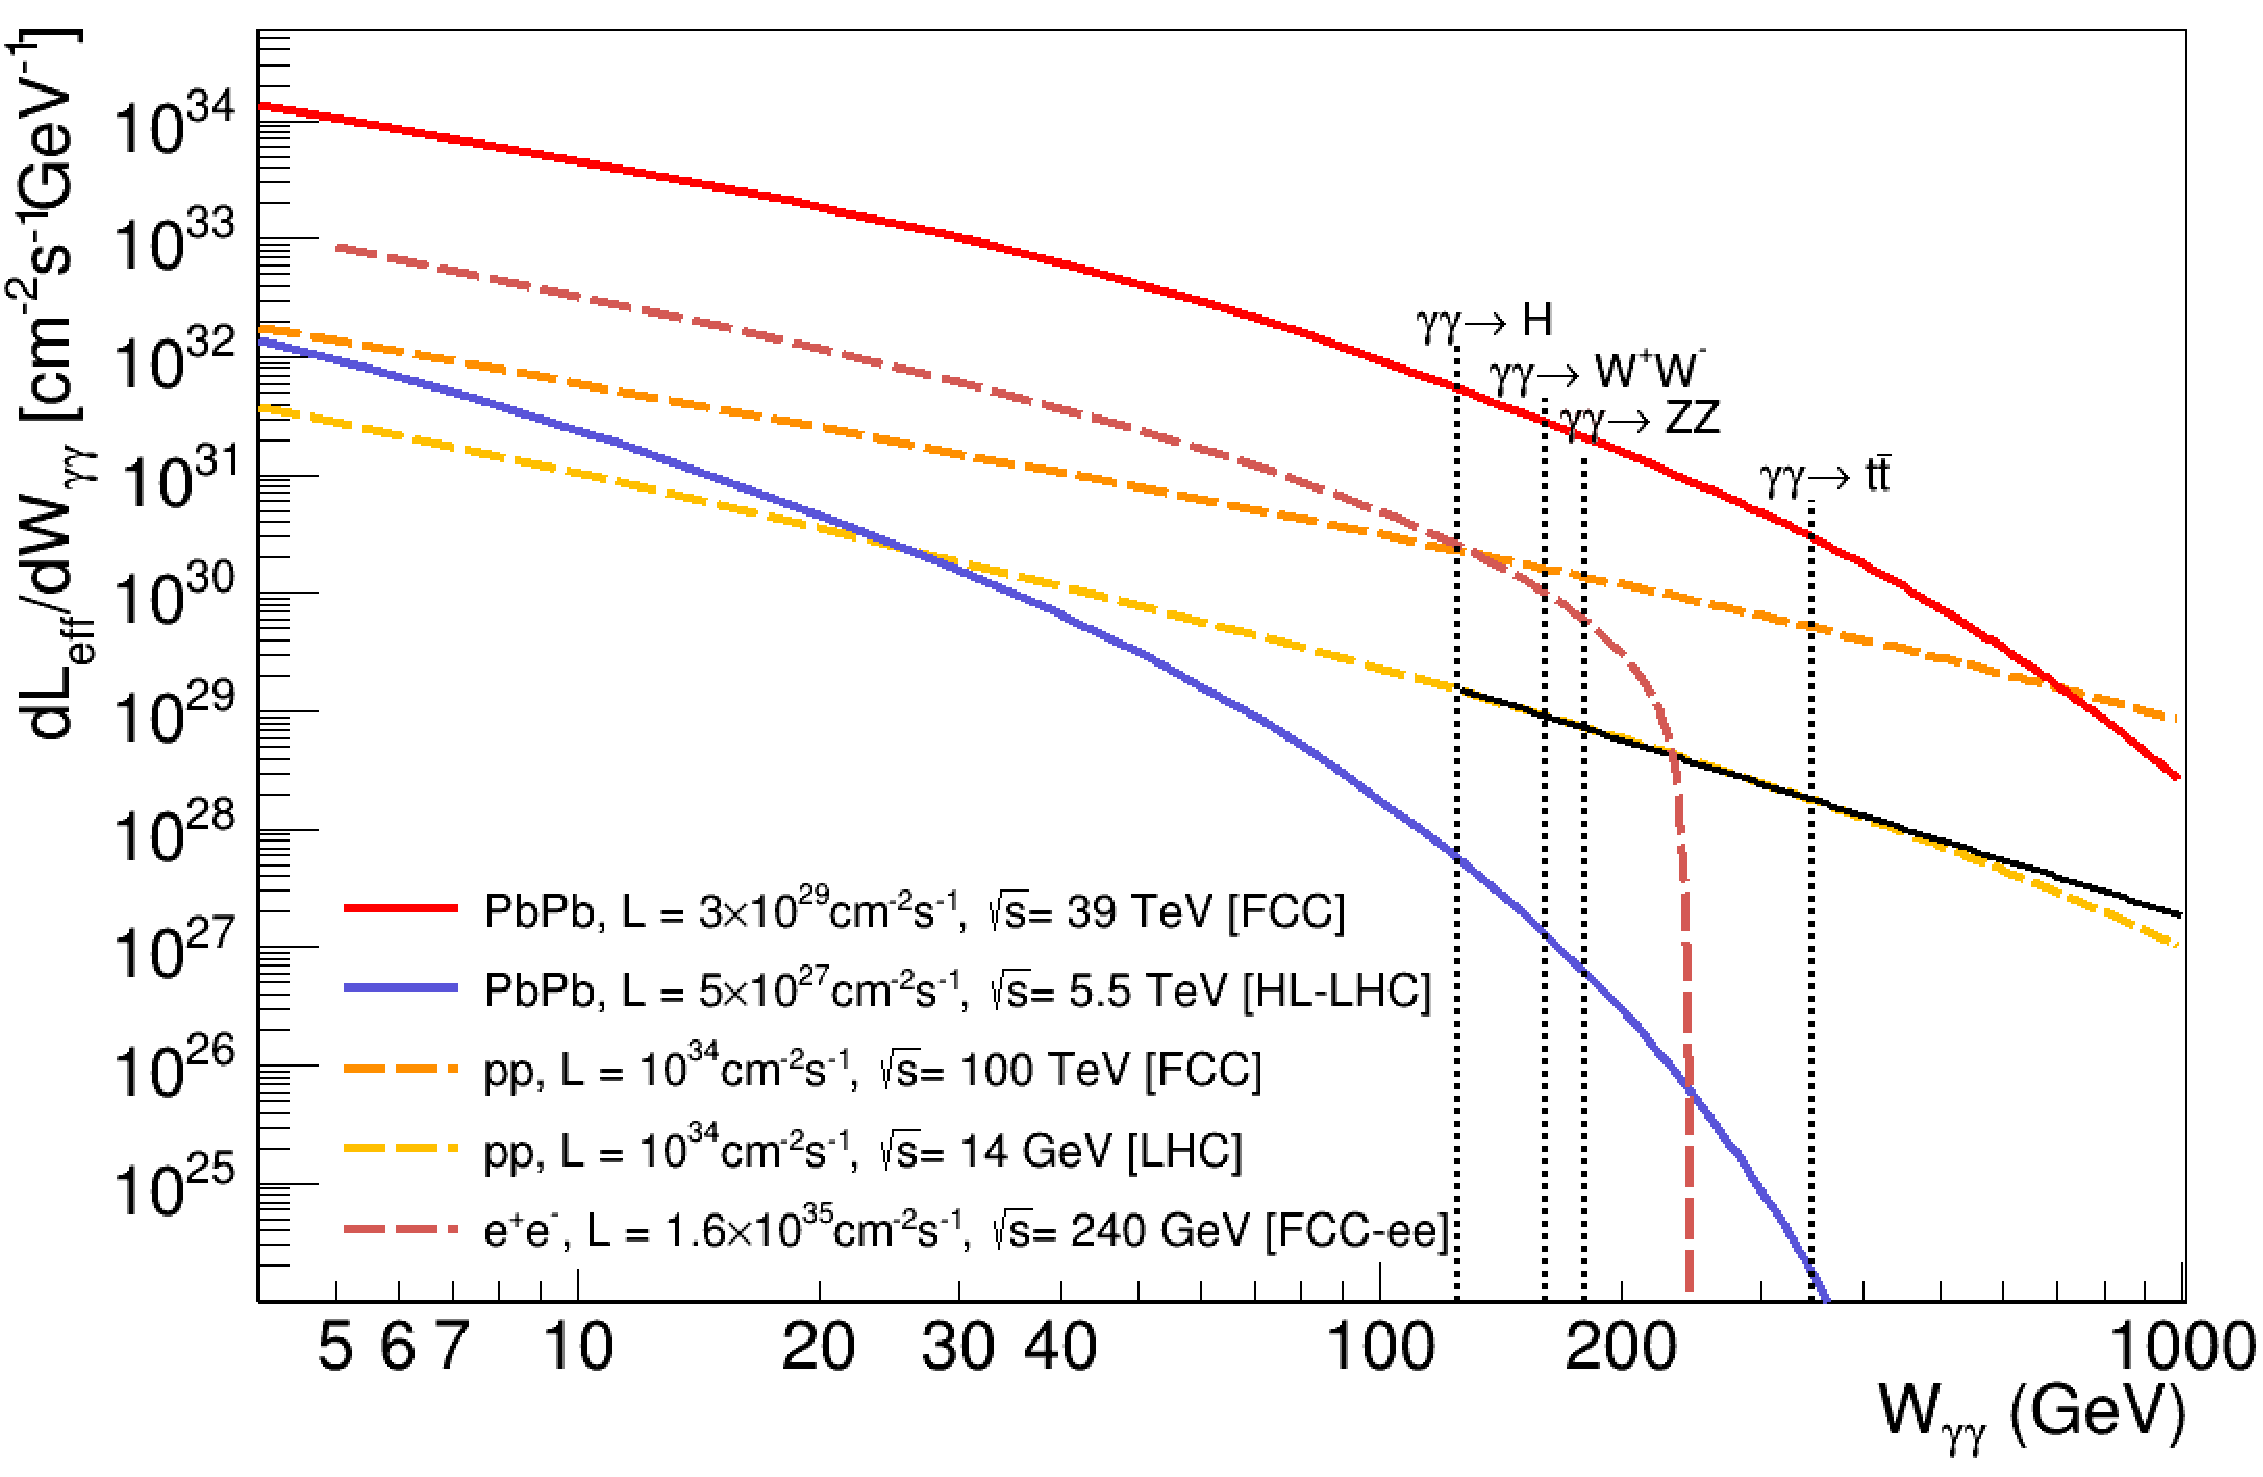
\includegraphics[width=0.52\columnwidth]{helhc/figs/lumi_gammagamma_fcc_ions.pdf}
%\includegraphics[width=0.45\columnwidth]{figs/PbPb_UPC_FCC_higgs_bbar_minv.pdf}
\caption{{\bf Curves for HE-LHC to be added.} Effective luminosities as a function of $\gaga$ centre-of-mass energy ($W_{\gaga}$) for five
  colliding systems at FCC and LHC energies and their nominal
  luminosities.}
\label{fig:gamgam_lumi}
\end{figure}


Photon--photon collisions in UPCs of proton~\cite{d'Enterria:2008sh} 
and lead (Pb) beams~\cite{Baltz:2007kq} have been experimentally observed at the
LHC~\cite{Chatrchyan:2012tv,Chatrchyan:2013foa,Abbas:2013oua,Aad:2015bwa}.
Although the $\gamma$ spectrum is harder for smaller charges --which favours proton over nuclear beams in the
production of heavy diphoton systems-- each photon flux scales with the squared charge of the hadron, $Z^2$, and
thus $\gaga$ luminosities are extremely enhanced for ion beams
($Z^4=5\cdot 10^{7}$ in the case of
\PbPb). 
The figure of merit for UPC $\gaga$ processes is the effective $\gaga$ luminosity, 
$\dd\mathcal{L}_{\rm eff}/\dd W_{\gaga} \equiv
\mathcal{L}_{AB}\,\dd\mathcal{L}_{\gaga}/\dd W_{\gaga}$, where ${\cal L}_{\rm AB}$ is the
collider luminosity for the $A$\,$B$ system and
$\dd\mathcal{L}_{\gaga}/\dd W_{\gaga}$ is the photon--photon luminosity
as a function of the $\gaga$ centre-of-mass energy $W_{\gaga}$, obtained integrating the two photon fluxes over all
rapidities $y$.
Figure~\ref{fig:gamgam_lumi} shows a comparison of the $\dd\mathcal{L}_{\rm eff}/\dd W_{\gaga}$ reachable as a
function of $W_{\gaga}$ for five different colliding systems at LHC,
{\bf HE-LHC} and FCC energies. Two-photon centre-of-mass
energies at the HE-LHC will reach for the first time the range beyond 0.5~TeV. 
The
vertical lines in Fig.~\ref{fig:gamgam_lumi} (left) show the thresholds for photon-fusion production of Higgs,
$W^+W^-$, $Z\,Z$, and $t\bar t$, which are sensitive to different tests of the electroweak sector of
the Standard Model (SM)~\cite{dEnterria:2017qte}, such as anomalous quartic-gauge couplings and top-electroweak
moments.


The very rare elastic scattering of two photons in vacuum
$\gaga\to\gaga$  was recently
observed for the first time in UPCs at the LHC~\cite{Aaboud:2017bwk,CMS-PAS-FSQ-16-012}.
{\bf The increase in $\gaga\to\gaga$ yields from LHC to HE-LHC is of $\mathcal{O}(200)$ thanks to factors
of $\times 30$ larger cross sections times luminosities, and $\times 2$ in the experimental acceptance~\cite{d'Enterria:2013yra,d'Enterria:2016qsv}. 
At the HE-LHC, due to the higher diphoton masses
reached, this process may be sensitive to physics beyond the SM through new heavy charged particles contributing to the
virtual loop such as, \eg\ from SUSY
particles~\cite{Gounaris:1999gh}. Light-by-light (LbyL) scattering has also been proposed as a tool to
search for monopoles~\cite{Ginzburg:1998vb}, axions~\cite{Bernard:1997kj}, unparticles~\cite{Kikuchi:2008pr}, 
low-scale gravity effects~\cite{Cheung:1999ja}, and non-commutative interactions~\cite{Hewett:2000zp}.}





% \subsection{Fixed-target collisions using the FCC proton and lead beams}
% \label{sec:HI_fixedtarget}


 
% \newcommand{\glabcms}{\gamma^{\rm lab}_{\rm c.m.s.}}
% \newcommand{\blabcms}{\beta^{\rm lab}_{\rm c.m.s.}}
% \newcommand{\dylabcms}{\Delta y^{\rm lab}_{\rm c.m.s.}}


% The fixed-target mode offers specific advantages compared to the collider mode 
% such as accessing the high Feynman $x_F$ domain, achieving high luminosities 
% yet in parasitic way, varying the atomic mass of the target almost at will, 
% and polarising the target~\cite{Lansberg:2015pra,Dainese:2016gch}.  
% The c.m.s.\,energy
% in the fixed-target mode is about 200--300~GeV for Pb and proton
% beams, respectively. 
% The region of central c.m.s.\,rapidities is highly 
% boosted at an angle with respect to the beam axis of about one degree 
% in the laboratory frame such that the entire backward hemisphere, $y_{\rm c.m.s.}<0$, becomes 
% easily accessible with standard experimental techniques at $2<\eta_{\rm lab} <6$. 
% A fixed-target setup would allow one to significantly extend a large number of measurements  
% carried out at RHIC towards very backward rapidities with much larger luminosities.
% As it was discussed in~\cite{Lansberg:2015pra}, RHIC luminosities in $pp$ collisions at 200~GeV are limited and
% could not allow for the study of vector boson production close to
% threshold which probes
% the large $x$ content in the proton and nucleus, 0.7 and above. 
% These studies become possible with with fixed-target collisons at FCC. 
% With a longitudinally polarised target, vector boson production gives access
% to (anti)quark helicity distributions in the proton at very large $x$. With deuterium and helium targets, measurements 
% can also be carried out on the neutron. Using a transversely polarised target allows one
% to access transverse-momentum dependent distributions (TMDs) which are connected to the orbital angular momentum carried
% by the partons at larger scales than with any other facilities.
% Given the similarities with a setup like AFTER@LHC, we also guide the reader to 
% Refs.~\cite{Brodsky:2012vg} for more in-depth discussions
% on the physics reach of the fixed-target mode above the 100~GeV domain.







\end{document}
